
%%%%%%%%%%%%%%%%%%%%%%%%%%%%%%%%%%%%%%%%%
% Beamer Presentation
% LaTeX Template
% Version 1.0 (10/11/12)
%
% This template has been downloaded from:
% http://www.LaTeXTemplates.com
%
% License:
% CC BY-NC-SA 3.0 (http://creativecommons.org/licenses/by-nc-sa/3.0/)
%
%%%%%%%%%%%%%%%%%%%%%%%%%%%%%%%%%%%%%%%%%

%----------------------------------------------------------------------------------------
%	PACKAGES AND THEMES
%----------------------------------------------------------------------------------------

\documentclass[10pt,xcolor={usenames,dvipsnames,table}]{beamer}

\mode<presentation> 
\usetheme{default}
\usecolortheme{orchid}
\usefonttheme{professionalfonts}
% \setbeamertemplate{note page}[plain]
% \setbeameroption{show notes on second screen=left}

\usepackage{graphicx} % Allows including images
\usepackage{booktabs} % Allows the use of \toprule, \midrule and \bottomrule in tables
\usepackage{algorithm}
\usepackage{algpseudocode}
\usepackage{multirow}
\usepackage{tikz}
\usetikzlibrary{calc}
\usetikzlibrary{arrows,automata}
\usetikzlibrary{positioning}
\usetikzlibrary{decorations.text}
\usetikzlibrary{decorations.pathmorphing}
\usepackage[english]{babel}
\usepackage{amsmath}
\usepackage[colorinlistoftodos]{todonotes}
\usepackage{algorithm}
\usepackage{algpseudocode}
\usetikzlibrary{tikzmark,calc}
\usepackage{mathtools}
\usepackage{amsthm}
%\usepackage{enumitem}

\usepackage[english]{babel}
\usepackage{listings}
\lstset{language=python}
\definecolor{codegreen}{rgb}{0,0.6,0}
\definecolor{codegray}{rgb}{0.5,0.5,0.5}
\definecolor{codepurple}{rgb}{0.58,0,0.82}
\definecolor{backcolour}{rgb}{0.95,0.95,0.92}

\lstdefinestyle{mystyle}{
    backgroundcolor=\color{backcolour},   
    commentstyle=\color{codegreen},
    keywordstyle=\color{magenta},
    numberstyle=\tiny\color{codegray},
    stringstyle=\color{codepurple},
    basicstyle=\ttfamily\footnotesize,
    breakatwhitespace=false,         
    breaklines=true,                 
    captionpos=b,                    
    keepspaces=true,                 
    numbers=left,                    
    numbersep=5pt,                  
    showspaces=false,                
    showstringspaces=false,
    showtabs=false,                  
    tabsize=2
}
\lstset{style=mystyle}
\usepackage[utf8]{inputenc}
\usepackage{csquotes}
\usepackage[citestyle=authoryear-comp,maxnames=1,uniquelist=false]{biblatex}
\addbibresource{refs.bib}
\usepackage{caption}
\usepackage{subcaption}
% \usepackage[hidelinks]{hyperref}
% \hypersetup{colorlinks,citecolor=blue,linkcolor=blue}
\usepackage{import}
\usepackage{xifthen}
\usepackage{pdfpages}
\usepackage{transparent}
\usepackage{bm}
\usepackage{tikz}
\usepackage{pgfplots}
\usepackage{hhline}
% --------------------------------------------------------- 
% SETTINGS
% --------------------------------------------------------- 
\counterwithin{figure}{section}
\newcommand\mycommfont[1]{\footnotesize\ttfamily\textcolor{blue}{#1}}
\definecolor{codegreen}{rgb}{0,0.6,0}
\beamertemplatenavigationsymbolsempty
\setbeamertemplate{footline}[page number]{}
\captionsetup{justification=centering,font=scriptsize}

\newrobustcmd*{\parentexttrack}[1]{%
  \begingroup
  \blx@blxinit
  \blx@setsfcodes
  \blx@bibopenparen#1\blx@bibcloseparen
  \endgroup}

\AtEveryCite{%
  \let\parentext=\parentexttrack%
  \let\bibopenparen=\bibopenbracket%
  \let\bibcloseparen=\bibclosebracket}
% --------------------------------------------------------- 
% CUSTOM COMMANDS
% --------------------------------------------------------- 

\def\green{\color{ForestGreen}}
\def\red{\color{red}}
\def\blue{\color{blue}}
\newcommand{\rank}[1]{\text{rank}(#1)}
\newcommand{\pr}[1]{\text{Pr}\left(#1\right)}
\newcommand{\st}{\text{subject to}\quad }
\newcommand{\trace}[1]{\text{tr}\left(#1\right)}
\newcommand{\norm}[1]{\left\lVert#1\right\rVert}
\newcommand{\abs}[1]{\left\lvert#1\right\rvert}
\newcommand{\vect}[1]{\text{vec}\left(#1\right)}
\newcommand{\diag}[1]{\text{diag}\left(#1\right)}
\newcommand\numberthis{\addtocounter{equation}{1}\tag{\theequation}} % https://tex.stackexchange.com/questions/42726/align-but-show-one-equation-number-at-the-end 
\newcommand{\set}[1]{\left\{#1\right\}}
\newcommand*\diff{\mathop{}\!\mathrm{d}}
\newcommand{\T}{\!\top\!}

\newcommand{\incfig}[2][1]{%
    \def\svgwidth{#1\columnwidth}
    \import{./figures/}{#2.pdf_tex}
}

\DeclareMathOperator*{\argmax}{arg\,max}
\DeclareMathOperator*{\argmin}{arg\,min}
\DeclareMathOperator*{\minimize}{minimize}
\DeclareMathOperator*{\maximize}{maximize}
% to change colors
\newcommand{\fillcol}{green!10}
\newcommand{\bordercol}{black}

\newcommand\DrawBox[3][]{%
  \begin{tikzpicture}[remember picture,overlay]
    \draw[overlay,fill=gray!30,#1] 
    ([xshift=-8em,yshift=2.1ex]{pic cs:#2}) 
    rectangle 
    ([xshift=2pt,yshift=-0.7ex]pic cs:#3);
  \end{tikzpicture}%
}
\newcommand*{\captionsource}[2]{%
  \caption[{#1}]{%
    #1%
    \\\hspace{\linewidth}%
    \textbf{Source:} #2%
  }%
}
\algnewcommand\algorithmicinput{\textbf{Input:}}
\algnewcommand\INPUT{\item[\algorithmicinput]}
\newcounter{saveenumi}
\newcommand{\seti}{\setcounter{saveenumi}{\value{enumi}}}
\newcommand{\conti}{\setcounter{enumi}{\value{saveenumi}}}
\newcommand{\indep}{\perp \!\!\! \perp}

\newcommand{\highlight}[1]{%
  \colorbox{red!50}{$\displaystyle#1$}}

\newcommand{\higreen}[1]{%
  \colorbox{green!40}{$\displaystyle#1$}}

\newcommand{\citep}[1]{{\blue \scriptsize \parencite{#1}}}
\newcommand{\citepb}[1]{{\scriptsize \parencite{#1}}}

% For matrix decoration
\newcommand\coolover[2]{\mathrlap{\smash{\overbrace{\phantom{%
    \begin{matrix} #2 \end{matrix}}}^{\mbox{$#1$}}}}#2}

\newcommand\coolunder[2]{\mathrlap{\smash{\underbrace{\phantom{%
    \begin{matrix} #2 \end{matrix}}}_{\mbox{$#1$}}}}#2}

\newcommand\coolleftbrace[2]{%
#1\left\{\vphantom{\begin{matrix} #2 \end{matrix}}\right.}

\newcommand\coolrightbrace[2]{%
\left.\vphantom{\begin{matrix} #1 \end{matrix}}\right\}#2}

% Highlight with Tikz
\usetikzlibrary{fit}
\tikzset{%
  highlight/.style={rectangle,rounded corners,fill=red!15,draw,
    fill opacity=0.5,thick,inner sep=0pt}
}
\newcommand{\tikzmarkx}[2]{\tikz[overlay,remember picture,
  baseline=(#1.base)] \node (#1) {#2};}
%
\newcommand{\Highlight}[1][submatrix]{%
    \tikz[overlay,remember picture]{
    \node[highlight,fit=(left.north west) (right.south east)] (#1) {};}
}
% --------------------------------------------------------- 
% CUSTOM ENVIRONMENTS
% --------------------------------------------------------- 
% \theoremstyle{plain}
% \newtheorem{theorem}{Theorem}[section]
\newtheorem{proposition}{Proposition}
%
% \theoremstyle{definition}
% \newtheorem{definition}{Definition}[section]
% \newtheorem{corollary}{Corollary}[theorem]
%
% \theoremstyle{remark}
% \newtheorem{remark}{Remark}[section]


%----------------------------------------------------------------------------------------
%	TITLE PAGE
%----------------------------------------------------------------------------------------

\title[Frank-Wolfe approach for Separable NMF]{Memory Efficient with Frank-Wolfe Method for Separable Nonnegative Matrix Factorization} % The short title appears at the bottom of every slide, the full title is only on the title page

\author{ Tri Nguyen} % Your name
\institute[OSU] % Your institution as it will appear on the bottom of every slide, may be shorthand to save space
{Qualifying Exam \\
Oregon State University \\ % Your institution for the title page
% \medskip
% \textit{nguyetr9@oregonstate.edu \endgraf } % Your email address
% }
}
\date{\today} % Date, can be changed to a custom date


\makeatletter
\makeatother


\begin{document}
%------------------------------------------------
\begin{frame}
\titlepage % Print the title page as the first slide
\note{
Hello everyone,
My name is Tri Nguyen. Today I'm glad to present my work for my qualifying exam. This work has been done with collaboration with 2 other researcher Dr. Wu and my advisor Prof. Fu.
}
\end{frame}
%------------------------------------------------
%------------------------------------------------

%------------------------------------------------
%\begin{frame}
%\frametitle{Contents} % Table of contents slide, comment this block out to remove it
%\tableofcontents % Throughout your presentation, if you choose to use \section{} and \subsection{} commands, these will automatically be printed on this slide as an overview of your presentation
%\end{frame}
%------------------------------------------------
%------------------------------------------------

%----------------------------------------------------------------------------------------
%	PRESENTATION SLIDES
%----------------------------------------------------------------------------------------
\includeonlyframes{current}

\section{Outline}
\begin{frame}
    \tableofcontents
    \note{
        \begin{itemize}
            \item A brief outline of the talk. We'll go through 4 parts. In the first section, I'll introduce the problem, elaborate the setting, and show some examples why we are interested in it.
            \item Then a quick look at how this problem has been solved. Particularly, there are 2 related different approaches, and we'll see what are their drawback and what could we offer to improve.
            \item In the third part, we advocate using an optimization method named Frank-Wolfe. 
                We'll try to show our intuition and rationale behind the proposal.
        \item Lastly, we showcase performance of the proposal via \textbf{both} synthetic experiment and real data experiments.
        \end{itemize}
    }
\end{frame}

\section{Problem of Interest}%

\subsection{Problem Setting}%
\label{sub:separable_nmf}


\begin{frame}
    \frametitle{Simplex Structure Matrix Factorization}

    {
\setbeamercolor{block title}{bg=BurntOrange,fg=black}
    \begin{block}{Simplex Structure Matrix Factorization (SSMF)}
    Data matrix $\bm{X} \in \mathbb{R}^{N \times M}$ is assumed to be generated by $\bm{W} \in \mathbb{R}^{N \times K}, \bm{H} \in \mathbb{R}^{K \times M}, \min(M, N) \gg K$  such that
    \[
    \bm{X} = \bm{W} \bm{H} + \bm{V} \quad \text{\rm subject to } \bm{H} \geq 0 , \bm{1}^{\T}\bm{H} = \bm{1}^{\T}
    \] 
    \end{block}}
    % In addition, $\bm{W}$ is assumed to be full rank.
    \begin{itemize}
        \item Closely related to nonnegative matrix factorization.
            
Since $\bm{W} \geq 0$, the constraint $ \bm{1}^{\T}\bm{H}= \bm{1}^{\T}$ can always be enforced by normalizing $\bm{X}$.
    \end{itemize}

    \begin{block}
        
    Given $\bm{X}$, how to find the ground truth $\bm{W}, \bm{H}$?
    \end{block}
    % \begin{figure}[t]
    %     \begin{subfigure}[t]{0.25\textwidth}
    %         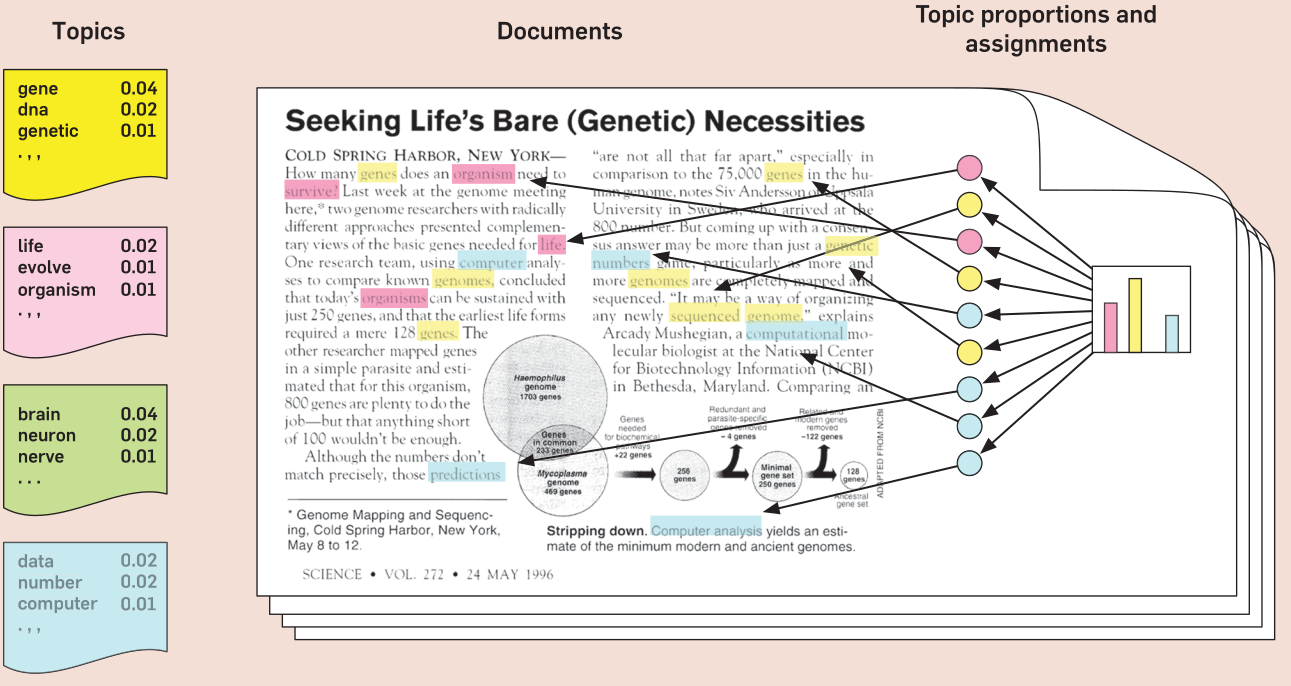
\includegraphics[width=\textwidth]{figures/topic_modeling_blei2021.png}
    %         \caption*{Topic modeling \citep{blei2012probabilistic}}
    %     \end{subfigure}
    %     \begin{subfigure}[t]{0.25\textwidth}
    %         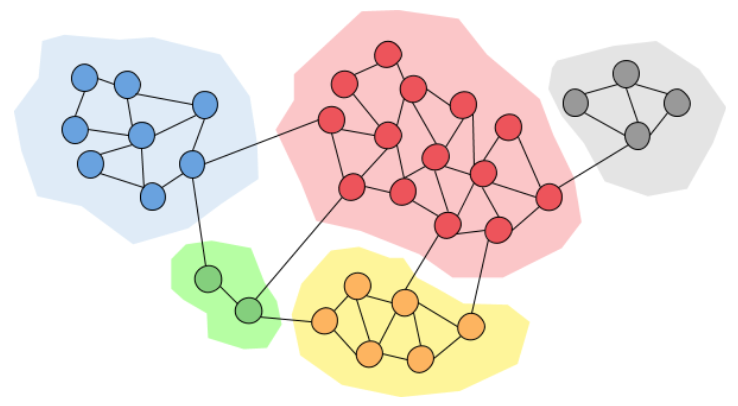
\includegraphics[width=\textwidth]{figures/comm_detection_internet.png}
    %         \caption*{Community detection}
    %     \end{subfigure}
    %     \begin{subfigure}[t]{0.23\textwidth}
    %         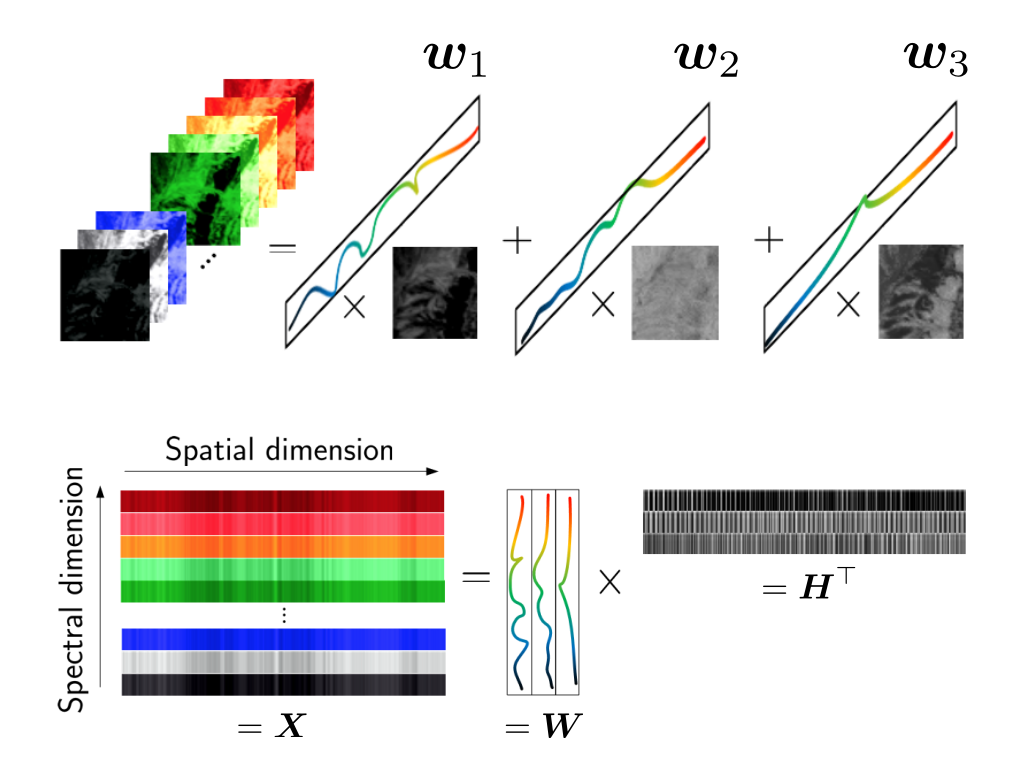
\includegraphics[width=\textwidth]{figures/hyperspectral_xiao2018.png}
    %         \caption*{Hyperspectral unmixing \citep{fu2018nonnegative}}
    %     \end{subfigure}
    %     \begin{subfigure}[t]{0.23\textwidth}
    %         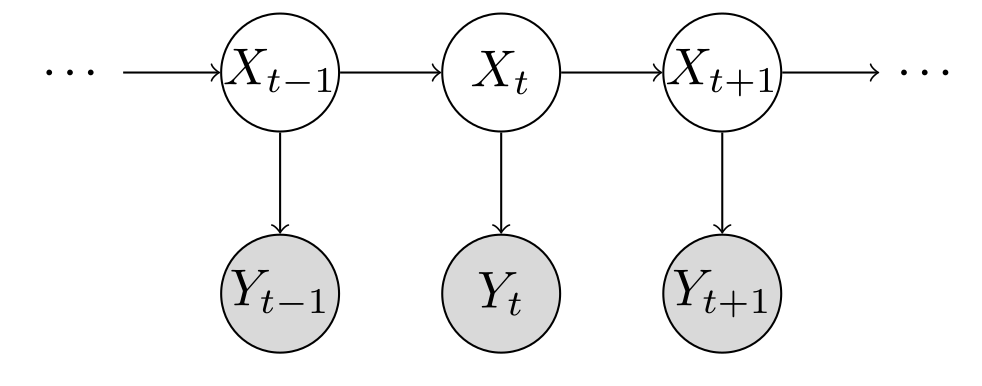
\includegraphics[width=\textwidth]{figures/hmm_xiao2018.png}
    %         \caption*{Hidden Markov Model \citep{fu2018nonnegative}}
    %     \end{subfigure}
    % \end{figure}
    % todo: these captions are too ugly
    % todo: check if hmm has simplex constraint

    \note{
    \begin{itemize}
        \item {\blue First Point}
        \item We are interesting a branch of matrix factorization, namely simplex structure matrix factorization. 
        \item In particular, the model assumes that the data matrix $\bm{X}$ is generated as a production of 2 low-rank matrix $\bm{W}, \bm{H}$. The inner dimension $K$ is assumed to be relatively small compared to $M, N$. 
        \item In addition, it is assumed that columns of $\bm{H}$ reside in a probability simplex. Note that we do not require nonnegativity on $\bm{W}$ as in NMF. 
        \item {\blue Second Point}
        \item This model are closely related to NMF in a sense that we can always convert a NMF model into SSMF model by performing a normalization on columns of $\bm{X}$. 
        
        \item {\blue Next} 
        \item What? So the problem is: Given $\bm{X}$, how do we find the ground truth $\bm{W}, \bm{H}$.
        \item Why? Finding $\bm{W}, \bm{H}$ is meaningful as they carries physical meaning depending on particular applications.
    \end{itemize}
}
\end{frame}

% \begin{frame}
%     \frametitle{Application: Topic Modeling}
%     \begin{figure}[t]
%         \centering
%         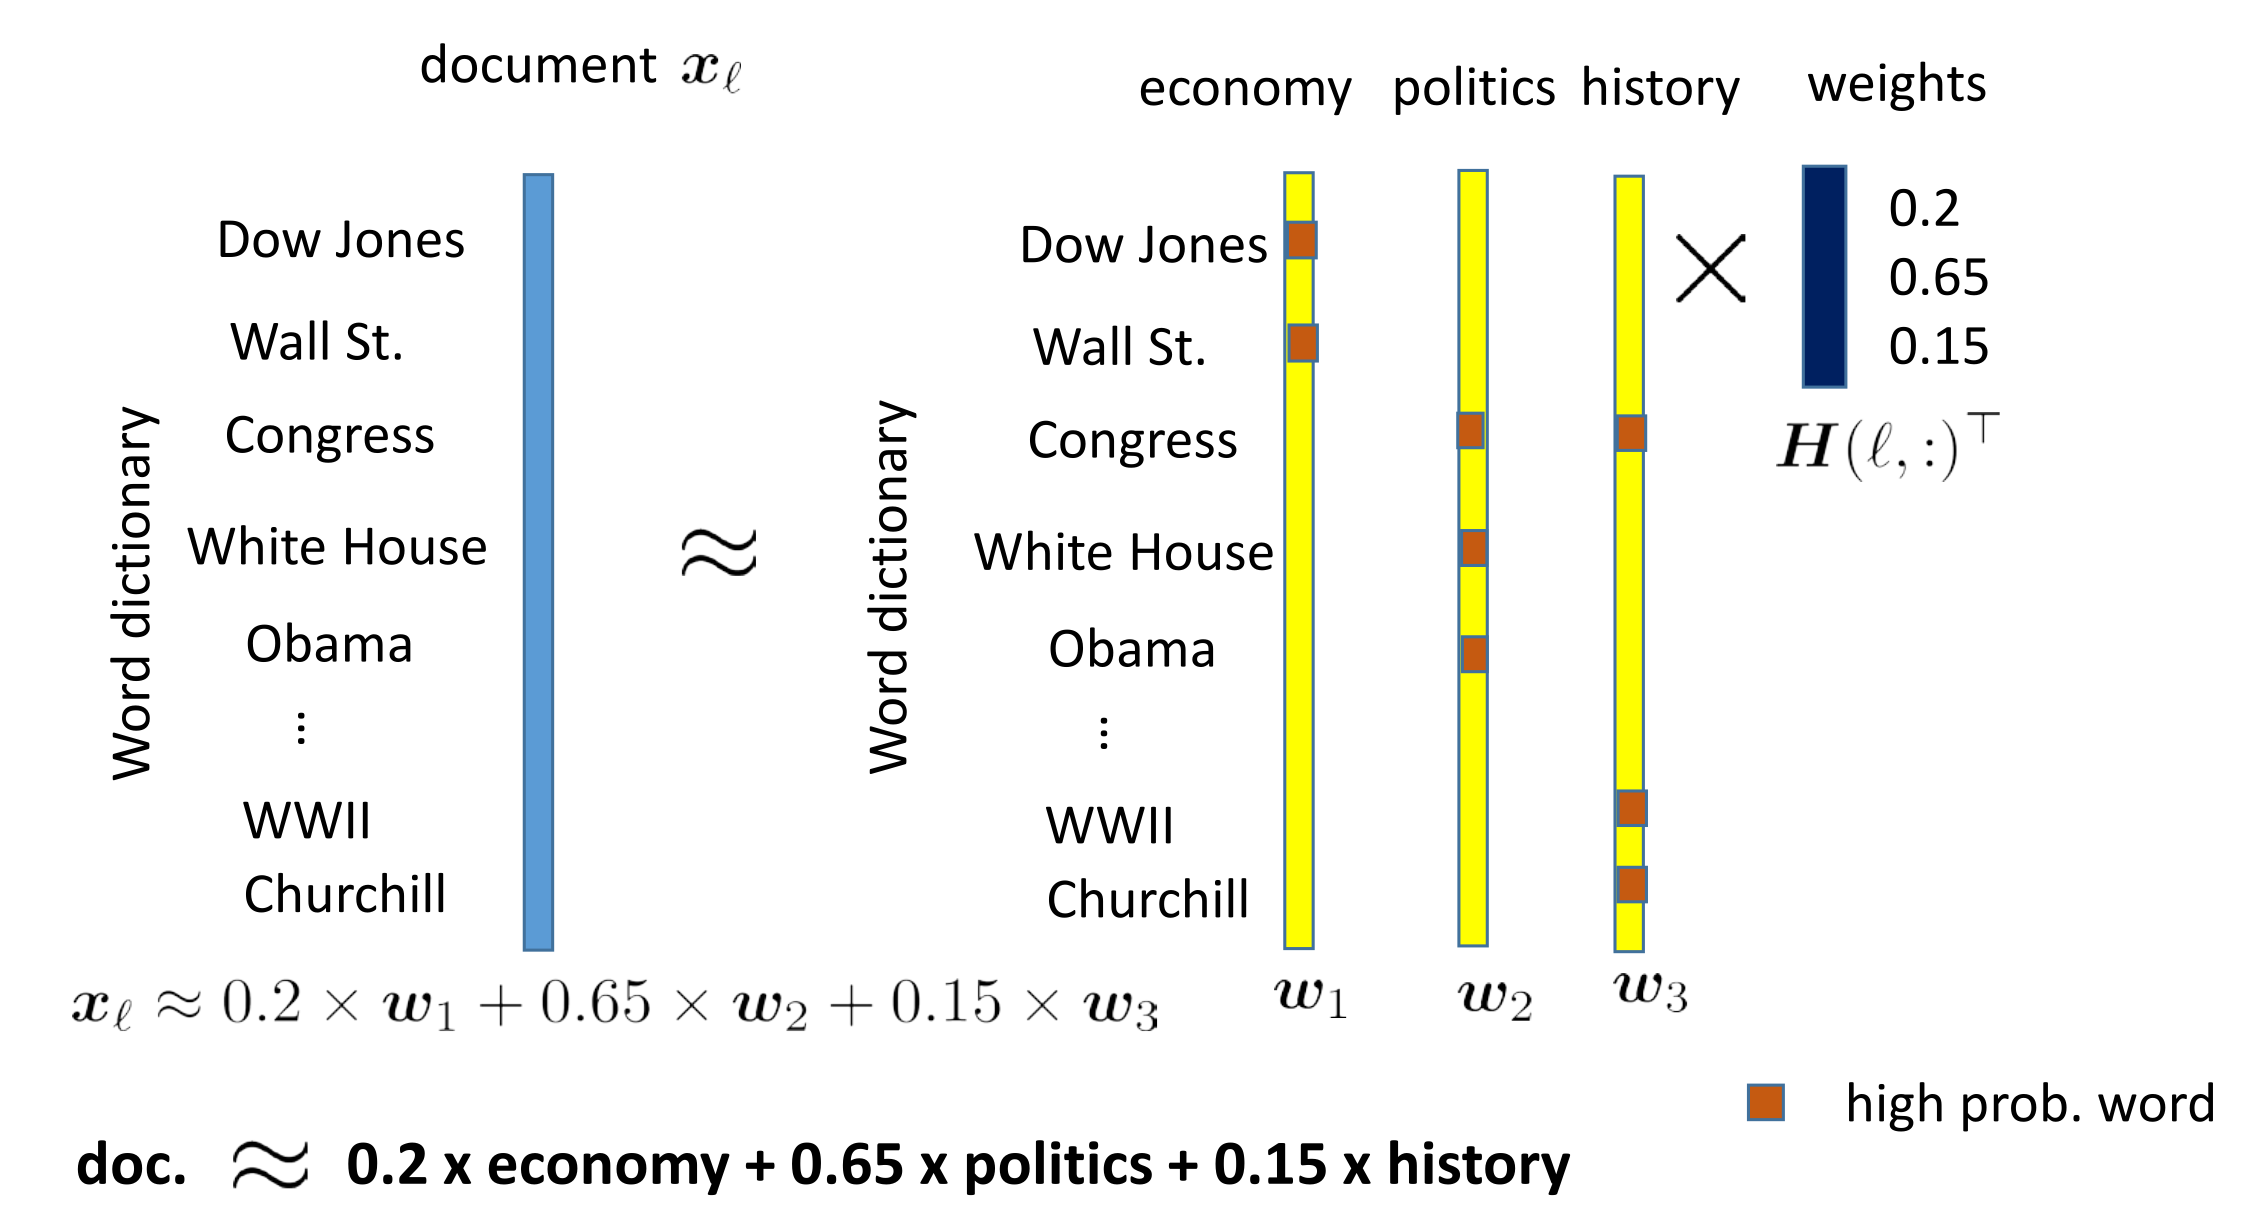
\includegraphics[width=0.8\textwidth]{figures/topic_modeling_demo.png}
%         \caption{A demonstration of $\bm{x}_\ell = \bm{W}\bm{h}_\ell$ {\red figure issue}}
%     \end{figure}
%
% % \begin{figure}[ht]
% %     \centering
% %     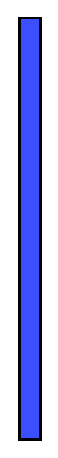
\includegraphics[width=0.1\textwidth]{figures/topic_modeling_demo.eps}
% %     \caption{sad}
% %     \label{fig:topic_modeling_demo}
% % \end{figure}
%     $\bm{X}$ is a vocab-document matrix, then $\bm{X} = \bm{W}\bm{H}$ where 
%     \begin{itemize}
%         \item $\bm{H} \geq 0,\bm{1}^{\T}\bm{H} = \bm{1}^{\T} $ 
%         \item $K$ is number of topics
%     \end{itemize}
%     
%     \note{ 
%     \begin{itemize}
%         \item In topic modeling, if data matrix $\bm{X}$ is a vocab-document matrix whose elements are some weights, then columns in $\bm{W}$ represents topics' signatures, and columns in $\bm{H}$ is a mixture of $F$ topics' signatures, then the topics of $\bm{X}$ can be though of a mixture of $F$ topics' signatures.
%     \end{itemize}
%     }
% \end{frame}
\subsection{Applications}%
\label{sub:applications}


\begin{frame}
    \frametitle{Application: Topic Modeling}
\begin{figure}[ht]
    \centering
    {
    \fontsize{7pt}{9pt}\selectfont% or whatever fontsize you like
    \def\svgwidth{\columnwidth}
    \import{./figures/}{topic_modeling_demo.pdf_tex}
    }
    \caption*{A demonstration of $\bm{x}_\ell \approx \bm{W} \bm{h}_\ell$}
\end{figure}
    $\bm{X}$ is a vocab-document matrix, then $\bm{X} = \bm{W}\bm{H}$ where 
    \begin{itemize}
        \item $\bm{H} \geq 0,\bm{1}^{\T}\bm{H} = \bm{1}^{\T} $ 
        \item $K$ is number of topics
    \end{itemize}
    
    \note{ 
    \begin{itemize}
        \item For example, in topic modeling, given a set of documents, it is desirable to cluster all documents into some small set of topics. It is reasonable to assume that a document is a mixture of a set of topics regarding to some representation. 
        \item Specifically, if data matrix $\bm{X}$ is a vocab-document matrix whose elements are some weights such as term-frequency, then list of topics could be represented by some vectors, in this case, $\bm{w}_1, \bm{w}_2, \bm{w}_3$ as 3 topics: economy, politics, and history.
        And document represented by $\bm{x}_\ell$ is nothing but a linear combination of these 3 topics, with some coefficients $\bm{h}_\ell$. Naturally, coefficients are sum-up-to 1 in this case.

    \item Hence, being able to identify $\bm{W}, \bm{H}$ not only help in clustering task, it also give an insight about how a topic is represented. 
    \item If we could identify $\bm{w}$s as in the figure, we could discover that topic economy are more associated with `Down Jones' , and `Wall St.' than the other words in dictionary. So in a way, we know what constitute a topic.
    \end{itemize}
    }
\end{frame}

\begin{frame}
    \frametitle{Application: Community Detection}
    \begin{columns}
        \begin{column}{0.7\textwidth}
    \begin{itemize}
        \item The mixed membership stochastic blockmodels \citep{airoldi2008mixed}
    \begin{align*}
    &P_{i,j} = \bm{h}_i^{\T} \bm{B} \bm{h}_j \\
    & \bm{A}(i,j) = \bm{A}(j, i) \sim \text{Bernoulli}(\bm{P}(i, j))
    \end{align*} 
    where $\bm{h}_i= [h_{1,i}, \ldots , h_{K, i}]^{\T}$ represents membership of node $i$, $\bm{B}$ represents community-community connection.
    \end{itemize}
        \end{column}
        \begin{column}{0.3\textwidth}
        \begin{figure}
            \centering
    \resizebox{\textwidth}{!}
            { 
            \incfig{community-detection-demo} }
            \caption*{Demonstration of a graph with $K=2$ communities}
        \end{figure}
        \end{column}
    \end{columns}

    \begin{columns}
        \begin{column}{1.\textwidth}
    \begin{itemize}
    \item By physical interpretation, $\bm{H} \geq 0, \bm{1}^{\T}\bm{H}=\bm{1}^{\T}$.
    \item Range space of $\bm{H}$ can be estimated via a constructed $\bm{X} \in \mathbb{R}^{K \times N}$ from $K$ leading eigenvectors of  $\bm{A}$.
        \citep{mao2017mixed,panov2018consistent} 
        \[
        \bm{X} = \bm{W} \bm{H} + \bm{N}
        \] 
    \end{itemize}
        \end{column}
    \end{columns}
    \note{
        \begin{itemize}
            \item Another application is community detection, where given a graph, we wish to discovery a small number of community constituted by set of nodes that are more connected to each other.
            \item As a well-known model, the mixed membership stochastic blockmodels models the probability of having a connection between node $i$ and $j$ by 2 parts:
                \begin{itemize}
                    \item  vector  $\bm{h}_i$ represents the membership of node $i$, and .
                    \item matrix $\bm{B}$ explains the interaction between communities
                \end{itemize}
            \item Note that the model is explicitly allowed overlapping communities as a node can belong to different communities at the same time.
            \item As a membership vector, it is natural that $\bm{h}$ is in a probability simplex.
            \item The issue is we only observe adjacency matrix $\bm{A}$ instead of the connection probability $\bm{P}$. An insight from these works suggest that
                by construct $K$ leading eigenvectors from  $\bm{A}$, we can approximate range space of $\bm{H}$, as the formulation
            \item This is nothing but the SSMF as we saw earlier.
        \end{itemize}
    }
\end{frame}

\begin{frame}
\frametitle{Identifiability}
\begin{itemize}
    % \item SSMF model with $\bm{X}, \bm{W}^{\star}, \bm{H}^{\star}$
    \item Given a SSMF model with $\bm{X} = \bm{W}^{\star} \bm{H}^{\star}$, one way to estimate $\bm{W}^{\star}, \bm{H}^{\star}$ is considering the following criterion
\begin{subequations}
    \label{problem:criteria}
\begin{alignat}{2}
    & \text{find}  && \quad \bm{W}, \bm{H} \\
    & \text{subject to } &&  \bm{X} = \bm{W}\bm{H} \\
    &&& \bm{H} \geq 0, \bm{1}^{\T}\bm{H} = \bm{1}^{\T}
\end{alignat}
\end{subequations}
\item The solution is not unique. There exists non-singular $\bm{Q}$ such that
\[
\bm{X} = \bm{W}^{\star} \bm{H}^{\star} = (\underbrace{\bm{W}^{\star}\bm{Q}^{-1}}_{\bm{W}'}) (\underbrace{\bm{Q} \bm{H}^{\star}}_{\bm{H}'}), \text{ and } \bm{H}' \geq 0, \bm{1}^{\T}\bm{H}' = \bm{1}^{\T}
\] 
% \item In topic modeling, each column in $\bm{W}^{\star}$ is believed to represent topics. However, the sought $\bm{W}'$ is some mixture of topics
\begin{definition}[Identifiability \citepb{fu2018nonnegative}]
    A SSMF model where $\bm{X}= \bm{W}^{\star} \bm{H}^{\star}$ is called identifiable respect to criterion \eqref{problem:criteria} if 
for all $\bm{W}, \bm{H}$ satisfying criterion \eqref{problem:criteria}, it holds that
    $\bm{W}=\bm{W}^{\star} \boldsymbol \Pi , \bm{H} = \boldsymbol \Pi^{\T}\bm{H}^{\star} $, where $\boldsymbol \Pi$ is a permutation matrix.
\end{definition}
\end{itemize}

\note{
\begin{itemize}
    \item There are several criteria that can be used to find $\bm{W}, \bm{H}$. The most straightforward is perhaps constructing the following optimisation problem where we're assuming there is no noise, thus the inequality constraint.
    \item Note that we do not just want to explain $\bm{X}$ with some matrices $\bm{W}, \bm{H}$. What we really want is finding the ground truth $\bm{W}^{\star}, \bm{H}^{\star}$.
    \item Unfortunately, the solution of Problem 1 is not unique. We can see why. It is trivial to construct $\bm{Q}$ \ldots 
    \item $\bm{W}', \bm{H}'$  in this case would not bring much useful information. For example, in topic modeling , $\bm{W}^{\star}$ represent the topics, while the sought $\bm{W}'$ represent a mixed of topics. Hence we haven't really got a good representation of topics by using $\bm{W}'$.
    \item By that reason, we narrow our interest to those models whose can be identified. In particular, by saying SSMF model is identifiable we mean that if criterion (1) has solution $\bm{W}, \bm{H}$ , then they are just some permutation of the ground truth.
    \item This kind of ambiguity is unharmed.
    \item The definition is borrowed from this work and modified to our specific SSMF problem.
\end{itemize}}

\end{frame}

\begin{frame}
\frametitle{Separability Condition}
\begin{block}{Separability condition}
    There exists set $\mathcal{K}$ so that $\bm{H}^{\star}(:, \mathcal{K}) = \bm{I}$. 
\end{block}
\begin{itemize}
    % \item Enabling identifiability of SSMF
    % \item Enabling polynomial algorithm
    \item Physical interpretation
\begin{itemize}
    \item Anchor word \citep{arora2012learning} in topic modeling
    \item Pure node \citep{mao2017mixed} in community detection
\end{itemize}
\begin{figure}[ht]
    \centering
    \begin{subfigure}[b]{0.55\textwidth}
    \centering
    \resizebox{\textwidth}{!}{
    \fontsize{4pt}{6pt}\selectfont% or whatever fontsize you like
    \def\svgwidth{\columnwidth}
    \import{./figures/}{anchor-word-demo.pdf_tex}
    }
    \caption*{Demonstration of anchor word}
    \end{subfigure}
    \begin{subfigure}[b]{0.30\textwidth}
    \centering
    { \fontsize{7pt}{9pt}\selectfont% or whatever fontsize you like
    \def\svgwidth{\columnwidth}
    \import{./figures/}{pure-node-demo.pdf_tex} }
    \caption*{Demonstration of pure node}
    \end{subfigure}
\end{figure}

\item Finding $\mathcal{K}$ is the key to estimate ground truth $\bm{W}^{\star}, \bm{H}^{\star}$.

    \begin{itemize}
        \item In noiseless case, $\bm{X}(:, \mathcal{K}) = \bm{W}^{\star} \bm{H}^{\star}(:, \mathcal{K}) = \bm{W}^{\star}$.
    \end{itemize}
\end{itemize}

\note{
\begin{itemize}
    \item So we will need more to have identifiability. There are several conditions that can guarantee identifiability. One of the well-known is separability condition.
    \item It states that \ldots 
    \item The condition is not only help guaranteeing identifiability but also has interesting and reasonable physical interpretation.
        \begin{itemize}
            \item For example, in topic modeling, it asserts that for each topic, such as economy, there exists a word that only belong to that topic, in this case, `Wall St.'. Similar to other topics.
            \item In communities, a node can belong to multiple communities. Under separability condition, there exists nodes called pure nodes, that only belong to a single community.
        \end{itemize}
    \item Moreover, this condition has been exploited in terms of algorithms. Particularly, the problem of finding $\bm{W}, \bm{H}$ boils down to finding the set $\mathcal{K}$. The rationale is like this.

        Consider a noiseless case, the sub-matrix $\bm{X}(:, \mathcal{K})$ that is constructed by stacking columns of $\bm{X}$ that has indices from $\mathcal{K}$.

    \item We drop the star notation when referring to ground truth to make notations light.
\end{itemize}}
\end{frame}

\section{Related Works}%
\label{sec:what_have_people_done_}

\begin{frame}
    \frametitle{A Self-Dictionary Perspective}
    \begin{columns}
    \begin{column}{0.8\textwidth}
    In noiseless case, the following 4 tasks are equivalent (under some regularity conditions)
    \begin{enumerate}
        \item Finding $\mathcal{K}$
        \item Finding set of vertices of $\text{conv}(\bm{W})$
        \item Finding a smallest set of columns in $\bm{X}$ to represent whole data $\bm{X}$
        \item  Optimizing
            \begin{subequations}
                \label{problem:self-dictionary}
                \begin{alignat}{2}
                    & \minimize_{\bm{C}} \quad && \norm{\bm{C}}_{\text{row-0}}  \\
                    & \text{\rm subject to} && \bm{X} = \bm{X} \bm{C} \\
                    &&& \bm{C} \geq 0, \bm{1}^{\T}\bm{C} = \bm{1}^{\T}
                \end{alignat}
            \end{subequations}
    % where $\norm{\bm{C}}_{\text{row-0}} := \sum^{N}_{n=1} \norm{\bm{C}(n, :)}_0$.
    \vspace{-0.5cm}
    \begin{itemize}
        \item $\bm{C}_{\text{opt}}(\mathcal{K}, :) = \bm{H}, \bm{C}_{\text{opt}}(\mathcal{K}^{c}, :) = \bm{0}$ is a feasible point.
        \item $\norm{\bm{C}_\text{opt}} = K$.
        \item For a full rank $\bm{W}$, one needs at least $K$ data points to represent $\bm{X}$.
        \item See \citep{fu2014self}.
    \end{itemize}
    \end{enumerate}
    \end{column}
    \begin{column}{0.35\textwidth}
    % \vspace{1cm}
    \begin{figure}[t]
        \centering
        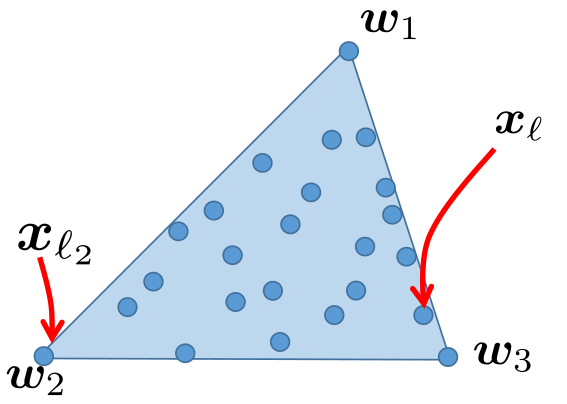
\includegraphics[width=0.6\textwidth]{figures/sdmmv_geometry.png}
        \caption*{$\bm{x}_\ell = \bm{W}\bm{h}_{\ell}$ \\ \citep{fu2018nonnegative}}

    \end{figure}

        \begin{figure}
            \centering
            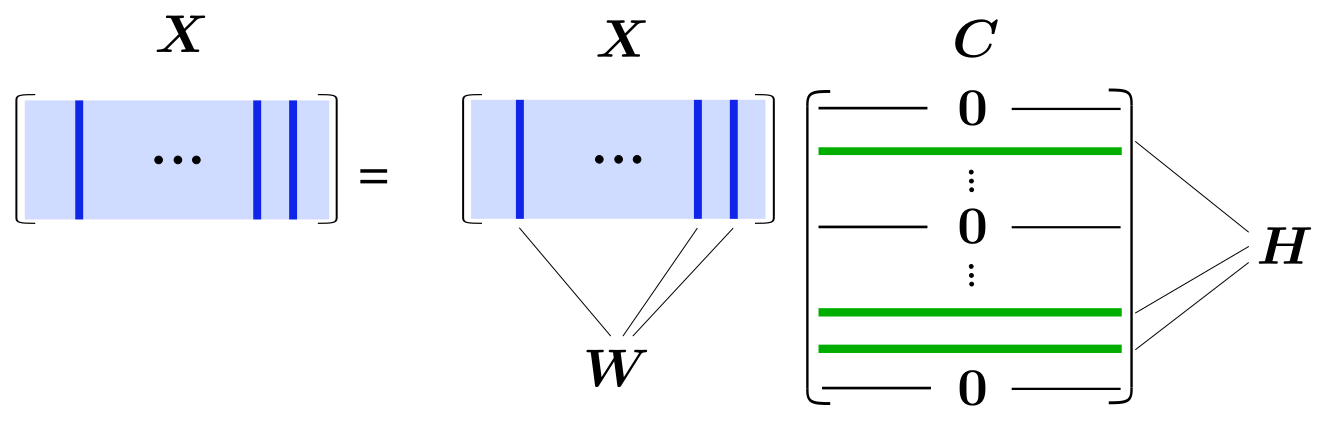
\includegraphics[width=\textwidth]{figures/sdmmv_demo/demo.png}
            \caption*{Row-sparsity matrix $\bm{C}$ }
        \end{figure}
    \end{column}
    \end{columns}


    \note{
    \begin{itemize}
        \item In noiseless case, the following 4 tasks are equivalent. Our primary goal is to find $\mathcal{K}$ as explained before
        \item As we have the probability simplex imposing on columns of $\bm{H}$, all columns $\bm{X}$ reside in convex hull of $\bm{W}$. And because of the separability condition, there are data points $\bm{x}_\ell$ that touch the vertices. These data points corresponds to indices in $\mathcal{K}$. That makes the tasks of finding $\mathcal{K}$ equivalent as allocating  vertices of the convex hull.
        \item And by convex property, finding vertices is equivalent to finding a smallest subset of points that can represent all data samples, since the vertices couldn't be represented by the others.
        \item Lastly, the task described in 3 can be formulated as the following optimisation problem, where the notation row-0 counts number of non-zero rows in $\bm{C}$
        \item We can see that one of the solution can be constructed  as follows. The rows corresponding to $\mathcal{K}$ is the ground truth $\bm{H}$, and the other rows are $ \bm{0}$.
        \item This is firstly a feasible point, as it satisfies all constraint.
        \item Secondly, for a full rank $\bm{W}$, one will need at least $K$ data points, hence this is an optimal solution.
        \item So by inspecting this $\bm{C}_{\text{opt}}$, we can identify $\mathcal{K}$ as indices of non-zero rows in $\bm{C}$
        \item A more rigorous proof can be found in this work.

        \item The formulation in (2) resembles dictionary learning, except that the dictionary is the data itself, hence the name self-dictionary.
            % To have a better look at this formulation, or how solving this formulation leads to $\mathcal{K}$? Next slide
    \end{itemize}}
% {  \setbeamercolor{block title}{bg=ForestGreen,fg=black}
%     \begin{block}
%
%          When $\text{rank}(\bm{W}) =K$, and assume $\mathcal{K}=[K]$, and noise is absent, then $\bm{C}_{\text{opt}} = \begin{bmatrix}
%          \bm{H} \\ \bm{0}
%          \end{bmatrix} $ since
%          $ \bm{X} \bm{C} = [\bm{W}, \bm{X}'] 
%          \begin{bmatrix}
%          \bm{H} \\ \bm{0}
%          \end{bmatrix}  = \bm{W}\bm{H} = \bm{X} $.
%
%          See formal proof at \citep{fu2014self}.
%     \end{block}
% }


\end{frame}

% \begin{frame}
%     \frametitle{A Self-Dictionary Perspective}
%     \begin{figure}[t]
%         \begin{subfigure}[b]{0.3\textwidth}
%         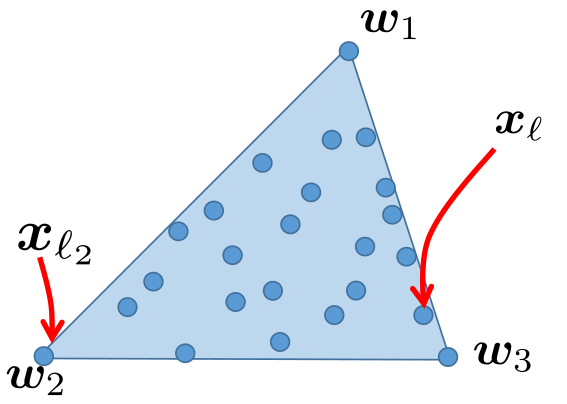
\includegraphics[width=\textwidth]{figures/sdmmv_geometry.png}
%         \caption*{$\bm{x}_\ell = \bm{W}\bm{h}_{\ell}$ \citep{fu2018nonnegative}}
%
%         \end{subfigure}
%         \quad \quad 
%         \begin{subfigure}[b]{0.55\textwidth}
%             \centering
%             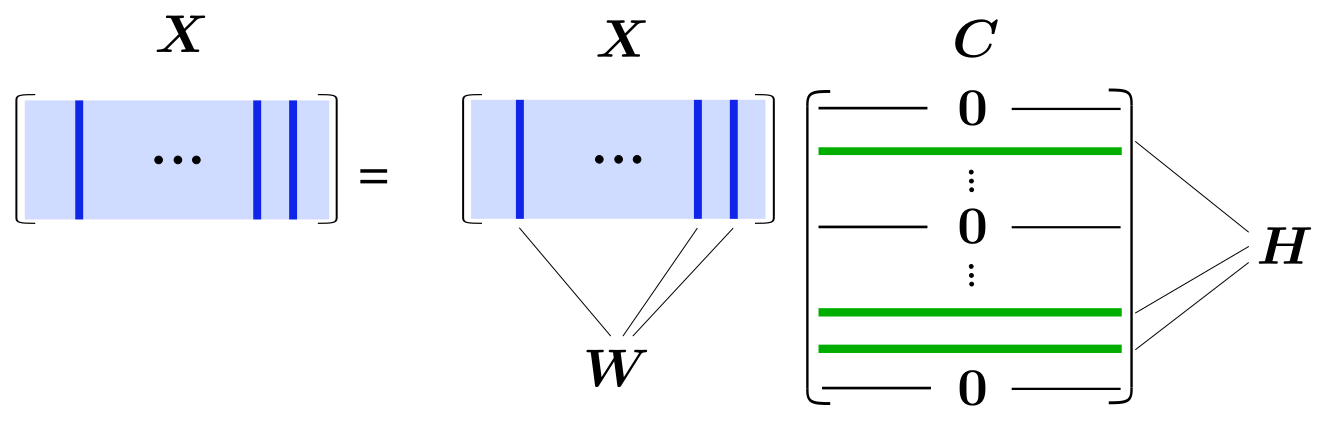
\includegraphics[width=\textwidth]{figures/sdmmv_demo/demo.png}
%             \caption*{Row-sparsity matrix $\bm{C}$ }
%         \end{subfigure}
%     \end{figure}
%     \begin{itemize}
%         \item Since $\bm{h}_\ell \geq 0, \bm{1}^{\T}\bm{h}_\ell=1$, then $\bm{x}_\ell \in \text{conv}(\bm{W})$
%         \item By separability assumption, there exist data points $\bm{x}_\ell$'s at the vertices of $\text{conv}(\bm{W})$
%         \item Hence, each column $\bm{x}_\ell$ is a convex combination of a small subset of columns in $\bm{X}$
% \item Self-dictionary with encouraging row-sparsity 
%     \end{itemize}
%     \begin{alignat*}{2}
%         & \minimize_{\bm{C}} \quad && \norm{\bm{C}}_{\text{row-}0} \\
%         & \text{\rm subject to} && \bm{X} = \bm{X} \bm{C} \\
%         &&& \bm{C} \geq 0, \bm{1}^{\T}\bm{C} = \bm{1}^{\T}
%     \end{alignat*}
%
%     % todo: change layout  to  | text | figure |
%
%     \note{
%     \begin{itemize}
%         \item We are looking for a basis in $\bm{X}$ to represent all columns in $\bm{X}$
%         \item To have a better look at this formulation, or how solving this formulation leads to $\mathcal{K}$? Next slide
%     \end{itemize}}
% \end{frame}

% \begin{frame}
%     \frametitle{A Self-Dictionary Perspective}
%     \begin{itemize}
%         \item Since columns of $\bm{H}$ belongs to a simplex, each column in $\bm{X}$ is a convex combination of $K$ columns of $\bm{W}$
%         \item By separability assumption, and assume that $\mathcal{K} = \set{1, 2, \ldots, N}$
%     \[
%     \bm{X} = \bm{W} \bm{H} = \bm{W} [\bm{I}, \bm{H}'] = [\bm{W}, \bm{W}\bm{H}']
%     \] 
% \item Hence, each column of $\bm{X}$ is a convex combination of a small subset of columns in  $\bm{X}$
% \item Self-dictionary with encouraging row-sparsity 
%     \end{itemize}
%     \begin{columns}
%         \begin{column}{0.3\textwidth}
%     \begin{alignat*}{2}
%         & \minimize_{\bm{C}} \quad && \norm{\bm{C}}_{\text{row-}0} \\
%         & \text{subject to} && \bm{X} = \bm{X} \bm{C} \\
%         &&& \bm{C} \geq 0, \bm{1}^{\T}\bm{C} = \bm{1}^{\T}
%     \end{alignat*}
%         \end{column}
%         \begin{column}{0.7\textwidth}
%             % \begin{figure}[t]
%             %     \centering
%             %     \def\svgwidth{\linewidth}
%             %     \import{./figures/sdmmv_demo}{demonstration.pdf_tex}
%             % \end{figure}
%         \end{column}
%     \end{columns}
%
%     \note{
%     \begin{itemize}
%         \item We are looking for a basis in $\bm{X}$ to represent all columns in $\bm{X}$
%         \item To have a better look at this formulation, or how solving this formulation leads to $\mathcal{K}$? Next slide
%     \end{itemize}}
% \end{frame}


\subsection{Greedy Approach}%
\label{sub:greedy_approach}



\begin{frame}
    \frametitle{Greedy Approach}
    \begin{alignat*}{2}
        & \minimize_{\bm{C}} \quad && \norm{\bm{C}}_{\text{row-}0} \\
        & \text{\rm subject to} && \bm{X} = \bm{X} \bm{C} \\
        &&& \bm{C} \geq 0, \bm{1}^{\T}\bm{C} = \bm{1}^{\T}
    \end{alignat*}
     \begin{itemize}
     % todo I want these 2 items to be in SD slide
     %     \item When $\text{rank}(\bm{W}) =F$, and assume $\mathcal{K}=\set{1, \ldots , N}$, and noise is absent, then $\bm{C}_{\text{opt}} = \begin{bmatrix}
     %     \bm{H} \\ \bm{0}
     %     \end{bmatrix} $ since
     %     \[
     %     \bm{X} \bm{C} = [\bm{W}, \bm{X}'] \begin{bmatrix}
     %     \bm{H} \\ \bm{0}
     %     \end{bmatrix}  = \bm{W}\bm{H} = \bm{X}
     %     \] 
     %
     % \item \citep{fu2015robust,esser2012convex} show similar idea for for noisy case.
         \item The greedy approach try to identify set $\mathcal{K}$ one index by a time by looking at columns in $\bm{X}$ \citep{gillis2014fast,fu2014self,nascimento2005vertex}
         \item Successive projection algorithm (SPA) \citep{MC01} as a representative. 
         \item Estimating exact $\mathcal{K}$ is guaranteed under noisy condition
         \item Gram-Schmidt like algorithm, which  is prone to error propagation
         % \item %todo the connection between the formulation and the method seems loose, read the All related paper
     \end{itemize}
     \note{
\begin{itemize}
    \item Solving this optimization problem is not a trivial task. It is firstly not a convex problem due to the row-0, and secondly, and more importantly, it is a combinatorial problem in essence. So a native greedy search would be prohibited even if number of vertices $K$ is given.
        \item One of the approach has been largely studied is greedy approach. As the name suggested, methods in this approach construct set $\mathcal{K}$ by adding 1 index at a time.
        \item A famous successive projection algorithm is a representitive.
        \item And estimating exact $\mathcal{K}$ is guaranteed, even under noisy condition.
        \item However, all methods in this approach has a Gram-Schidt-like structure in their algorithms. This is a weak point as it is prone to error propagation.
\end{itemize}
     }
\end{frame}


\subsection{Convex Relaxation Approach}%
\label{sub:convex_relaxation_approach}



\begin{frame}
    \frametitle{Convex Relaxation Approach}
    \begin{itemize}
        \item Relax the formulation to a convex optimization problem \citep{gillis2018afast,gillis2014robust,gillis2013robustness,recht2012factoring,Elhamifar2012,Ammanouil2014blind}
        \item An example of this approach is \citep{esser2012convex,fu2015robust}
    \begin{alignat*}{2}
        & \minimize_{\bm{C}} \quad && \dfrac{1}{2} \norm{\bm{X} - \bm{X}\bm{C}}_{\rm F}^2 + \lambda \norm{\bm{C}}_{\infty, 1} \\
        & \text{\rm subject to} && \bm{C} \geq 0, \bm{1}^{\T}\bm{C} = \bm{1}^{\T}
    \end{alignat*}
    where $\norm{\bm{C}}_{\infty, 1} := \sum^{N}_{n=1} \norm{\bm{C}(n, :)}_{\infty}$.
\item $\mathcal{K}$ is identified based on optimal $\bm{C}$
\item Often more robust than greedy approach
\item However, this approach suffers from large memory consumption
    \end{itemize}

    % \begin{alertblock}{Potential Memory Issue}
    %     The variable $\bm{C}$ has size $N \times N$
    % \end{alertblock}
    \begin{figure}
    \begin{tikzpicture}[scale=0.48]
        \begin{axis}[
            /pgf/number format/1000 sep={},
            xlabel=$N$,
            ylabel=Memory cost in RSS (GB),
            legend pos=north west,
            legend cell align={left},
            xticklabel style={
                    /pgf/number format/fixed,
            },
            scaled x ticks=false,
            % yticklabels={0, 1, 2, 3, 4, 5},
            extra y ticks={1, 3, 5, 6},
            % extra y tick labels={0.3, 5.0},
            % extra tick style={tickwidth=\pgfkeysvalueof{/pgfplots/minor tick length}},
            ]
        \addplot[orange,mark=o,only marks] table [x=N, y=FG]{figures/synthetic_data/exp2/mem.dat};
        \addplot[dashed,blue,domain=1000:10000, samples=5,] {0.000000055*x^2 - 0.000024*x + 0.12};
        \legend{\texttt{FastGradient}, curve $aN^2 + b N +c$}
        \end{axis}
    \end{tikzpicture}
    \caption*{Memory consumption of \texttt{FastGradient} \citep{gillis2018afast} grows in order of $O(N^2)$ }
% {\red consider add cvx figure}
    \end{figure}

    \note{
    \begin{itemize}
        \item The second approach try to identify $\mathcal{K}$ in all-at-once manner, so this avoids the accumulation error.
        \item As mentioned before, the original problem is non-convex, which make it hard in terms of optimisation. 
        \item So one way is to use a convex opt problem as a surrogate. There has been many convex relaxation formulations proposed in the literature. One example is this formulation where the row-0 is relaxed by the so-called mixed norm. 
        \item Under this formulation, identifiability is guaranteed via optimal solution $\bm{C}$.
        \item Since the algorithm does not suffer from error propagation, it is often more robust then the previous approach. We'll see some evidence on this in our experiments.
        \item However, memory is an obstacle for this approach. As we can see, size of variable $\bm{C}$ is $N$ by $N$.  If it is a dense matrix, memory requirement will grow quadratically.  
            As an example, we run a method named FastGradient from this work, which is considered as state-of-the-art under this approach, on a synthetic setting and measure its memory consumption. We can see that memory cost grows quadratically to $N$. This prohibits its applicability to large scale problem when  $N$ could reach to 100000.
        \item We aim to overcome this obstacle while retaining noise robustness advantage of this approach by proposing using Frank-Wolfe method.
        \item {\blue we can consider run another simulation for the formulation above}
    \end{itemize}
    }
\end{frame}


\section{Proposal: Frank-Wolfe}%
\label{sec:what_are_we_proposing_}

\subsection{Warm-up: Noiseless Case}%

% \begin{frame}[label=fine]
%     \frametitle{ Convex relaxation }
%     \begin{alignat*}{2}
%         & \minimize_{\bm{C}} \quad && \norm{\bm{X}  - \bm{X} \bm{C}}_{\rm F}^2 \\
%         & \text{subject to} && \bm{C} \geq 1, \bm{1}^{\T}\bm{C} = \bm{1}^{\T}
%     \end{alignat*}
%     While the desired $\bm{C}^{\star} = \begin{bmatrix}
%          \bm{H} \\
%          \bm{0}
%         \end{bmatrix} $ is one optimal solution, 
%     \begin{itemize}
%     \item There exist other optimal solutions. Additional constraints are imposed to rule them out, such as:
%         \begin{itemize}
%             \item Gillis: \ldots 
%             \item More constraints make the optimisation complicated.
%         \end{itemize}
%     \item Variable $\bm{C}$ has size of $N \times N$ that requires $O(N^2)$ memory.
%         \begin{itemize}
%             \item Reduce $N$
%             \item Gillis: Computation efficiency
%         \end{itemize}
%     \end{itemize}
%     W.T.L.G., assume 
%     \[
%     \mathcal{K} = \set{1, 2, \ldots , K} \Leftrightarrow \bm{H} = [\bm{I}, \bm{H}']
%     \] 
%     \note{
%         \begin{itemize}
%             \item Good news
%             \item Bad news
%             \item Prove the point of "having other solution" Tri
%             \item {\red moving the last assumption to the somewhere else!}
%         \end{itemize}
%     }
% \end{frame}

\begin{frame}
    \frametitle{Warm-up with Noiseless Case}
    \begin{subequations}
    \label{problem:noiseless_warmup}
    \begin{alignat}{2}
        & \minimize_{\bm{C}} \quad && \dfrac{1}{2} \norm{\bm{X} - \bm{X}\bm{C}}_{\rm F}^2  \\
        & \text{\rm subject to} && \bm{C} \geq 0, \bm{1}^{\T}\bm{C} = \bm{1}^{\T}
    \end{alignat}
    \end{subequations}
    Problem \eqref{problem:noiseless_warmup} can have several solutions
    \begin{itemize}
        \item A desired solution $\bm{C}^{\star}(\mathcal{K}, :) = \bm{H}, \bm{C}^{\star}(\mathcal{K}^{c}, :) = \bm{0}$
        \item A trivial solution $\bm{I}_{N}$
    \end{itemize}

    \begin{figure}[!t]
      \centering
      \begin{subfigure}[t]{0.3\textwidth}
      \centering
      \begin{tikzpicture}[scale=0.4]
          \begin{axis}[
              /pgf/number format/.cd,
              1000 sep={},
              xlabel=$n$,
              ylabel=$\norm{\bm{C}_{\text{opt}}(n, :)}$,
              legend pos=south east,
              legend cell align={left},
              ]
          \addplot+[only marks,
              mark=o,
              ] table [x=index, y=norm]{code/pgd_C.dat};
          \addplot+[only marks,
              mark=o,
              ] table [x=index, y=norm]{code/pgd_C_pure_pixel.dat};
          \legend{$n \notin \mathcal{K}$, $n \in \mathcal{K}$}
          \end{axis}
      \end{tikzpicture}
      \caption*{\texttt{APG - Objective value: $3.99{e-}5$}}
      \end{subfigure}
      \begin{subfigure}[t]{0.3\textwidth}
      \centering
      \begin{tikzpicture}[scale=0.4]
          \begin{axis}[
              /pgf/number format/.cd,
              1000 sep={},
              xlabel=$n$,
              ylabel=$\norm{\bm{C}_{\text{opt}}(n, :)}$,
              legend pos=south east,
              legend cell align={left},
              ]
          \addplot+[only marks,
              mark=o,
              ] table [x=index, y=norm]{code/fw_C.dat};
          \addplot+[only marks,
              mark=o,
              ] table [x=index, y=norm]{code/fw_C_pure_pixel.dat};
          \legend{$n \notin \mathcal{K}$, $n \in \mathcal{K}$}
          \end{axis}
      \end{tikzpicture}
      \caption*{\texttt{FW} - Objective value: $2.86{e-}5$}
      \end{subfigure}
      \begin{subfigure}[t]{0.3\textwidth}
      \centering
      \begin{tikzpicture}[scale=0.4]
          \begin{axis}[
              /pgf/number format/.cd,
              1000 sep={},
              xlabel=iter,
              ylabel=nnz($\bm{C}$),
              legend pos=north east,
              legend cell align={left},
              ]
          \addplot[orange] table [x=iter, y=PGD]{code/nnz_fw_pgd.dat};
          \addplot[blue] table [x=iter, y=FW]{code/nnz_fw_pgd.dat};
          \legend{\texttt{APG}, \texttt{FW}}
          \end{axis}
      \end{tikzpicture}
      \caption*{Number of nonzeros (nnz) of $\bm{C}$}
      \end{subfigure}
      \caption*{\texttt{Accelerated proximal gradient (APG)} vs \texttt{Frank-Wolfe (FW)}. Unlike \texttt{APG}, \texttt{FW} outputs exact $\bm{C}^{\star}$ and keeps $\bm{C}$ sparse during its procedure. $M=10, N=50, K=3$}
  \end{figure}  

  \note{
      \begin{itemize}
          \item To see how FW helps over memory issue, let's start with a noiseless case. Consider a simple optimisation problem. This problem is convex, but could have multiple solution.
          \item A desired solution $\bm{C}^{\star}$ is one of them. It is a desired solution because by inspecting $\mathcal{C}^{\star}$, we can extract $\mathcal{K}$ exactly.
          \item There are other solutions as well, for example, an identity matrix, which provides no information about $\mathcal{K}$.
          \item To demonstrate, we compare results when running Accelerated Proximal Gradient, a typical first order method for constrained optimisation problem, and compare it with Frank-Wolfe.
          \item As we can see, both methods converged and gives a good solutions in terms of objective value. However, only FW outputs a solution $\bm{C}^{\star}$ which is perferectly reveal $\mathcal{K}$.
          \item Moreover, and more interestingly, if we take a look at the density of $\bm{C}$ against iterations, we can see that FW consistently keeps $\bm{C}$ being very sparse, compared to APG. This is the key for memory efficiency when using FW.
      \end{itemize}
  }
\end{frame}

% \begin{frame}[label=fine]
%     \frametitle{Proposal: a Frank-Wolfe Approach}
%     \begin{subequations}
%     \label{problem:noiseless0}
%     \begin{alignat}{2}
%         & \minimize_{\bm{C}} \quad && \dfrac{1}{2} \norm{\bm{X} - \bm{X}\bm{C}}_{\rm F}^2  \\
%         & \text{\rm subject to} && \bm{C} \geq 0, \bm{1}^{\T}\bm{C} = \bm{1}^{\T}
%     \end{alignat}
%     \end{subequations}
% \begin{theorem}[Noiseless Case, Memory Efficiency] \label{theorem:noiseless}
%     %todo let the no repeated unit vectors a trap for questions
%     Suppose that 
%     \begin{itemize}
%         \item $\text{rank}(\bm{W})=K$, no repeated unit vectors exist in $\bm{H}$
%         \item The noise is absent (i.e., $\bm{V}=\bm{0}$)
%         \item Define $\bm{q}_\ell^t = \bm{W}^{\T}\bm{W}(\bm{H}\bm{c}_\ell^t - \bm{h}_\ell)$. Assume 
% \begin{align}\label{eq:nodupq}
%  q_{i,\ell}^t - \min_{j} q_{j,\ell}^t \neq 0,~\forall i \neq \argmin_{j} q_{j,\ell}^t,
% \end{align}
%     \end{itemize}
% Then, using FW  with initialization $\bm{C}^0 = \bm{0}$ to solve \eqref{problem:noiseless0} can reveal exact $\mathcal{K}$ using $O(KN)$ memory.
% \end{theorem}
%
% % \begin{block}{Fact}
% %     Condition \eqref{eq:nodupq} is almost guaranteed if $\bm{W}$ is drawn from some joint continuous distribution.
% % \end{block}
%
% \note{
% \begin{itemize}
%     \item Interesting result, 
%     \item Explain 4 assumptions, causally mention the triviality of the last assumption
%     \item Emphasize: get the right solution, while using less memory
%     \item {\blue Question: is using $\bm{C}=\bm{0}$ valid?}
%     \item {\blue check word "almost guarantee", is it the same as $P=1$.}
% \end{itemize}
% }
% \end{frame}


\begin{frame}
    \frametitle{Frank-Wolfe (FW) method \citep{jaggi2013revisiting}}
    For a convex function $f(\bm{x})$ and a compact convex constraint  $\mathcal{D}$ 
    \begin{alignat*}{2}
        & \minimize_{\bm{x}} \quad && f(\bm{x}) \\
        & \text{\rm subject to} && \bm{x} \in \mathcal{D}
    \end{alignat*}
    \begin{itemize}
        \item A standard procedure: at iteration $t$,
        \begin{align}
        &\bm{s}^{t} \leftarrow \argmin_{\bm{s} \in \mathcal{D}} \; \nabla f(\bm{x}^{t})^{\T} \bm{s} \label{eq:fw_general_update}\\
        &\bm{x}^{t+1} \leftarrow \bm{x}^{t} + \alpha^{t} (\bm{s}^{t} - \bm{x}^{t}) , \quad \alpha^{t}=2/(2+t) \nonumber
        \end{align}

        \item For $\mathcal{D} = \set{\bm{x} \in \mathbb{R}^{n} \mid \bm{x} \geq 0, \bm{1}^{\T}\bm{x} = 1}$, solving $\eqref{eq:fw_general_update}$ only costs $O(n)$.

    \[
    \bm{s} = \bm{e}_{n^{\star}}, \; n^{\star} = \argmin_{n} [\nabla f(\bm{x}^{t})]_n
    \] 
    % \item FW only update $n^{\star}$-th element of $\bm{x}$ per iteration.
    % \item With $\bm{x}^{0} = \bm{0}$, and $n^{\star} \in \mathcal{K}$, then $\text{supp}(\bm{x}^{t})=K$
% \item With an initialization $\bm{x}^{0} = \bm{0}$, Can we show $n^{\star} \in \mathcal{K}$?
    \end{itemize}
    
    \note{
    \begin{itemize}
        \item Conditional gradient descent
    \end{itemize}
    }
\end{frame}

% \begin{frame}
%     \frametitle{Revisit Frank-Wolfe}
%     Given a convex function $f$, a compact convex set  $\mathcal{C}$, FW solves 
%     \begin{alignat*}{2}
%         & \minimize_{\bm{x}} \quad &&  f(\bm{x}) \\
%         & \text{subject to} && \bm{x} \in \mathcal{D}
%     \end{alignat*}
%     with update procedure for $t=0, 1, \ldots $
%     \begin{align}
%         &\bm{s} \leftarrow  \min_{\bm{s} \in \mathcal{D}} \nabla f(\bm{x}^{t})^{\T} \bm{s} \\
%         &\bm{x}^{t+1} \leftarrow (1-\alpha^{t})\bm{x}^{t} + \alpha^{t} \bm{s}, \quad \text{for }  \alpha^{t} = \dfrac{2}{2+t}
%     \end{align}
%    \begin{itemize}
%        \item Does not involve a projection to $\mathcal{D}$.
%        \item Convergence rate $O(1/t)$ [x].
%        \item Scalability [x].
%    \end{itemize} 
% \note{\blue This one should be introduced earlier}
% \end{frame}

% \begin{frame}[label=fine]
%     \frametitle{FW in Noiseless Case}
%     \begin{itemize}
%         \item The objective w.r.t $\bm{c}_\ell$ (omitting $\ell$) is
%     $ f(\bm{c}) = \norm{\bm{X} - \bm{X}\bm{c}}_2^2 $
% \item The FW updates: $\bm{c}^{0} =\bm{0}$, for $t=1, 2, \ldots $
%     \begin{align}
%         &\bm{s} \leftarrow  \min_{\bm{s}\geq 0, \bm{1}^{\T}\bm{s}=1} \nabla f(\bm{c}^{t})^{\T} \bm{s} \label{eq:fw_linear} \\
%         &\bm{c}^{t+1} \leftarrow (1-\alpha^{t})\bm{c}^{t} + \alpha^{t} \bm{s}, \quad \text{for }  \alpha^{t} = \dfrac{2}{2+t}
%     \end{align}
% \item Since \eqref{eq:fw_linear} is a linear problem with a simplex constraint,
%     \[
%     \bm{s} = \bm{e}_{n^{\star}},\quad n^{\star} := \argmin_{n} \; [\nabla f(\bm{c}^{t})]_n
%     \] 
%     \end{itemize}
%     {
% \setbeamercolor{block title}{bg=ForestGreen,fg=black}
%     \begin{block}{ }
%     We will show that $n^{\star} \in \mathcal{K}$. And that leads to memory guarantee
%     \[
%         c_{n}^{t} = 0 \quad   \text{if } n \notin \mathcal{K}
%     \] 
%     \end{block}
%     }
%
%     \note{\blue same frame title, consider using title(1), title(2)}
% \end{frame}

\begin{frame}[label=fine]
    \frametitle{FW for Noiseless Case}
%     {
% \setbeamercolor{block title}{bg=ForestGreen,fg=black}
%     \begin{block}{}
%         Show that $ n^{\star} := \argmin_{n} \; [\nabla f(\bm{c}^{t})]_n \Rightarrow  n^{\star} \in \mathcal{K}$
%     \end{block}
%     }
The original problem can be solved for each column $\bm{c}$ independently
    \begin{alignat*}{2}
        & \minimize_{\bm{c} \in \mathbb{R}^{N}} \quad && \dfrac{1}{2} \norm{\bm{x} - \bm{X}\bm{c}}_{\rm F}^2 := f(\bm{c}) \\
        & \text{\rm subject to} && \bm{c} \geq 0, \bm{1}^{\T}\bm{c} = 1
    \end{alignat*}
    \begin{block}{Goal}
        Show that FW produces the desired solution $\bm{c}^{\star}(\mathcal{K}) = \bm{h}, \bm{c}^{\star}(\mathcal{K}^{c})= \bm{0}$ using $O(K)$ memory.
    \end{block}

    \begin{itemize}
    \item Initialize $\bm{c}^{0} =\bm{0}$
    \item  Updating rule
        \begin{align*}
        &\bm{s}^{t} = \bm{e}_{n^{\star}}, \; n^{\star} = \argmin_{n} [\nabla f(\bm{c}^{t})]_n \\
        &\bm{c}^{t+1} \leftarrow \bm{c}^{t} + \alpha^{t} (\bm{s}^{t} - \bm{c}^{t}) , \quad \alpha^{t}=2/(2+t)
        \end{align*}
    \item $n^{\star} \in \mathcal{K}$ holds for every steps
    \item When FW terminates, $\bm{c}_{\text{opt}}(\mathcal{K}^{c}) = \bm{0}, \bm{c}_\text{opt}(\mathcal{K}) = \bm{h}$
    \end{itemize}
\end{frame}

\begin{frame}
    \frametitle{FW on Noiseless Case}
    \begin{itemize}
        \item Gradient
    \begin{align*}
        \nabla f(\mathbf{c}) 
        =\bm{X}^{\T} (\bm{X}\bm{c} -\bm{x}) 
        = \bm{H}^{\T} \underbrace{\bm{W}^{\T}\bm{W} (\bm{H}\bm{c} - \bm{h}) }_{\bm{q}} 
        = [\bm{h}_1^{\T}\bm{q}, \ldots , \bm{h}_N^{\T}\bm{q}]^{\T}
    \end{align*}
    \item Lower bound
    \[
        [\nabla f(\bm{c})]_n =\bm{h}_n^{\T}\bm{q}
        \geq \left( \min_{j\in[ K]} q_{j} \right)  \sum^{K}_{j=1} h_{j,n} 
        = \min_{j\in[ K]} q_{j}
    \]
    Lower bound is obtained at $n^{\star}$ when either
    \begin{itemize}
        \item $\bm{h}_{n^{\star}} = \bm{e}_{k^{\star}}$, where $k^{\star} = \argmin_{k \in [K]} q_k$. By definition, $n^{\star} \in \mathcal{K}$.
        \item $\bm{q} = \bm{0} \Rightarrow$ optimal solution is found because
            \[
            \bm{q} = \bm{0} \Leftrightarrow
            \bm{H}\bm{c} = \bm{h} \Leftrightarrow \begin{bmatrix}
                \bm{I} & \bm{H}'
            \end{bmatrix}  \bm{c} = \bm{h}
            \Leftrightarrow \bm{c} = \begin{bmatrix}
            \bm{h} \\ \bm{0}
            \end{bmatrix} 
            \] 
    \end{itemize}
    \end{itemize}
\end{frame}

\begin{frame}
    \frametitle{FW on Noiseless Case}
    To summary,
    \begin{itemize}
        \item Only $c_{k}, k\in \mathcal{K}$ are updated, the others are $0$
        \item FW terminates when $\bm{c} = \begin{bmatrix}
        \bm{h} \\ \bm{0}
        \end{bmatrix}$
    \item Hence, memory used by FW is $O(KN)$ and FW outputs $\bm{C}_{\text{opt}} = \bm{C}^{\star}$
    \end{itemize}

    \begin{alertblock}
        
    When noise is introduced, solution $\bm{C}_{\texttt{opt}}$ would deviate away from $\bm{C}^{\star}$
    \end{alertblock}

    \begin{figure}[!t]
      \centering
      \begin{subfigure}[t]{0.32\textwidth}
      \centering
      \begin{tikzpicture}[scale=0.4]
          \begin{axis}[
              /pgf/number format/.cd,
              1000 sep={},
              xlabel=$n$,
              ylabel=$\norm{\bm{C}_{\text{opt}}(n, :)}$,
              legend pos=south east,
              legend cell align={left},
              ]
          \addplot+[only marks,
              mark=o,
              ] table [x=index, y=norm]{code/demo2_35_C.dat};
          \addplot+[only marks,
              mark=o,
              ] table [x=index, y=norm]{code/demo2_35_pure_pixel.dat};
          \legend{$n \in \mathcal{K}$, $n \in \mathcal{K}$}
          \end{axis}
      \end{tikzpicture}
      \caption*{\texttt{SNR}$=35$dB}
      \end{subfigure}
      \begin{subfigure}[t]{0.32\textwidth}
      \centering
      \begin{tikzpicture}[scale=0.4]
          \begin{axis}[
              /pgf/number format/.cd,
              1000 sep={},
              xlabel=$n$,
              ylabel=$\norm{\bm{C}_{\text{opt}}(n, :)}$,
              legend pos=south east,
              legend cell align={left},
              ]
          \addplot+[only marks,
              mark=o,
              ] table [x=index, y=norm]{code/demo2_25_C.dat};
          \addplot+[only marks,
              mark=o,
              ] table [x=index, y=norm]{code/demo2_25_pure_pixel.dat};
          \legend{$n \in \mathcal{K}$, $n \in \mathcal{K}$}
          \end{axis}
      \end{tikzpicture}
      \caption*{\texttt{SNR}$=25$dB}
      \end{subfigure}
      \begin{subfigure}[t]{0.32\textwidth}
      \centering
      \begin{tikzpicture}[scale=0.4]
          \begin{axis}[
              xlabel=$n$,
              % yticklabels={, 0.99, , , 1.00},
              ytick={0.99, 1.00},
              ylabel=$\norm{\bm{C}_{\text{opt}}(n, :)}$,
              legend pos=south east,
              legend cell align={left},
              ]
          \addplot+[only marks,
              mark=o,
              ] table [x=index, y=norm]{code/demo2_15_C.dat};
          \addplot+[only marks,
              mark=o,
              ] table [x=index, y=norm]{code/demo2_15_pure_pixel.dat};
          \legend{$n \in \mathcal{K}$, $n \in \mathcal{K}$}
          \end{axis}
      \end{tikzpicture}
      \caption*{\texttt{SNR}$=15$dB}
      \end{subfigure}
      \caption*{$\bm{C}_{\text{opt}}$ obtained by FW; $M=40, N=50, K=10$.}
  \end{figure}  
\end{frame}

\subsection{Enhancement for Noisy Case}%
\begin{frame}[label=fine]
    \frametitle{Enhancement for Noisy Case}
    \begin{itemize}
        \item Regularization has been used to promote row-sparsity \citep{fu2015robust,esser2012convex}
\[
\norm{\bm{C}}_{\infty, 1} = \sum^{N}_{i=1} \norm{\bm{C}(i, :)}_{\infty}
\] 
\item FW works best with smooth function 
    \[
    \varPhi_{\mu}(\bm{C}) = \sum^{N}_{i=1} \varphi_{\mu}(\bm{C}(i, :)) , \quad \varphi_{\mu}(\bm{C}(i, :)) = \mu \log \left( \dfrac{1}{N} \sum^{N}_{j=1} \exp \left(\dfrac{c_{i, j}}{\mu} \right) \right)
    \] 
\item We propose the formula
    \label{problem:noiseless}
    \begin{alignat*}{2}
        & \minimize_{\bm{C}} \quad && \dfrac{1}{2}\norm{\bm{X} - \bm{X}\bm{C}}_{\rm F}^2 + \lambda \varPhi_{\mu}(\bm{C}) \\
        & \text{\rm subject to} && \bm{C} \geq 0, \bm{1}^{\T}\bm{C} = \bm{1}^{\T}
    \end{alignat*}
    \end{itemize}

    \note{
    \begin{itemize}
        \item Comment on $\mu$
        \item ``In the end, we aim to solve \ldots ''
    \end{itemize}
    }
\end{frame}

\begin{frame}[label=fine]
    \frametitle{Identifiability}

    \begin{itemize}
        \item With regularization, extracting exact $\mathcal{K}$ is guaranteed via inspecting $\bm{C}_{\text{opt}}$ under some reasonable assumptions.
\begin{align*} 
    \|\bm{C}_{\text{opt}}(n,:)\|_\infty &> 1- \beta, ~ \forall n \in {\mathcal{K}}, \\
    \|\bm{C}_{\text{opt}}(n,:)\|_\infty &\leq 2\rho\dfrac{N-K}{ \lambda N} \norm{\bm{V}}_{\rm F}^2 + \mu N \log(N) + \beta K ,  ~~\forall n \notin {\cal K}  \\
&\beta = \dfrac{ \sqrt{4\rho (1-K/N) \norm{\bm{V}}_{\rm F}^2 + 2{ \lambda} K} + 2\delta } { \kappa(\bm{W})(1-d(\bm{H}))} 
\end{align*}
        \item Any convex optimization method can be used to obtain $\bm{C}_{\text{opt}}$
    \end{itemize}

    \begin{figure}[!t]
      \centering
      \begin{subfigure}[t]{0.32\textwidth}
      \centering
      \hspace{-1cm}
      \begin{tikzpicture}[scale=0.45]
          \begin{axis}[
              /pgf/number format/.cd,
              1000 sep={},
              xlabel=$n$,
              ylabel=$\norm{\bm{C}_{\text{opt}}(n, :)}$,
              legend pos=south east,
              legend cell align={left},
              ]
          \addplot+[only marks,
              mark=o,
              ] table [x=index, y=norm]{code/demo3_fw_C.dat};
          \addplot+[only marks,
              mark=o,
              ] table [x=index, y=norm]{code/demo3_fw_C_pure_pixel.dat};
          \legend{$n \in \mathcal{K}$, $n \in \mathcal{K}$}
          \end{axis}
      \end{tikzpicture}
      \caption*{\texttt{FW} - Objective value: $3.58{e-}01$}
      \end{subfigure}
      \begin{subfigure}[t]{0.32\textwidth}
      \centering
      \hspace{-0.5cm}
      \begin{tikzpicture}[scale=0.45]
          \begin{axis}[
              /pgf/number format/.cd,
              1000 sep={},
              xlabel=$n$,
              ylabel=$\norm{\bm{C}_{\text{opt}}(n, :)}$,
              legend pos=south east,
              legend cell align={left},
              ]
          \addplot+[only marks,
              mark=o,
              ] table [x=index, y=norm]{code/demo3_pgd_C.dat};
          \addplot+[only marks,
              mark=o,
              ] table [x=index, y=norm]{code/demo3_pgd_C_pure_pixel.dat};
          \legend{$n \in \mathcal{K}$, $n \in \mathcal{K}$}
          \end{axis}
      \end{tikzpicture}
      \caption*{\texttt{APG} - Objective value: $4.41{e-}01$}
      \end{subfigure}
      \begin{subfigure}[t]{0.32\textwidth}
      \centering
      \begin{tikzpicture}[scale=0.45]
          \begin{axis}[
              /pgf/number format/.cd,
              1000 sep={},
              xlabel=$n$,
              ylabel=$\norm{\bm{C}(n, :)}$,
              legend pos=south east,
              legend cell align={left},
              ]
          \addplot[orange] table [x=iter, y=FW]{code/demo3_nnz_fw_pgd.dat};
          \addplot[blue] table [x=iter, y=PGD]{code/demo3_nnz_fw_pgd.dat};
          \legend{\texttt{FW}, \texttt{APG}}
          \end{axis}
      \end{tikzpicture}
      \caption*{Number of nonzeros (nnz) of $\bm{C}$}
      \end{subfigure}
      \vspace{-0.3cm}
      \caption*{$M=40, K=10, N=50, \texttt{SNR}=30\text{dB}, \mu=1{e-}6, \lambda = 0.1$.}
  \end{figure}
\end{frame}
% \begin{theorem}[Identifiability]
%     \label{theorem:identifibility}
% Assume that 
% \begin{itemize}
%     \item $\text{rank}(\bm{W})=K$, no repeated unit vector in $\bm{H}$
%     \item $ \norm{\bm{v}_i}^2 \leq (\rho / N) \norm{\bm{V}}_{\rm F}^2$ for some $\rho$ and  $\norm{\bm{v}_i}_2 \leq \delta$
% \end{itemize}
% Then, any optimal solution $\bm{C}_{\rm opt}$ satisfies: 
% \begin{align*} 
%     \|\bm{C}_{\rm opt}(n,:)\|_\infty &> 1- \highlight{\beta}, ~ \forall n \in {\mathcal{K}}, \\
%     \|\bm{C}_{\rm opt}(n,:)\|_\infty &\leq 2\rho\dfrac{N-K}{ \higreen{\lambda} N} \norm{\bm{V}}_{\rm F}^2 + \higreen{\mu} N \log(N) + \highlight{\beta} K ,  ~~\forall n \notin {\cal K} \nonumber
% \end{align*}
% where 
% \begin{align*}
% &\beta = \dfrac{ \sqrt{4\rho (1-K/N) \norm{\bm{V}}_{\rm F}^2 + 2{ \lambda} K} + 2\delta } { \kappa(\bm{W})(1-d(\bm{H}))} 
% \end{align*} 
% \end{theorem}

% \begin{frame}
%     \frametitle{Identifiability}
%     From the previous,
%     \[
%     \beta = \dfrac{ \sqrt{4\rho (1-K/N) \norm{\bm{V}}_{\rm F}^2 + 2{\lambda} K} + 2\delta } { \kappa(\bm{W})(1-d(\bm{H}))} ,
%     \] 
%     where
% \begin{align*}
% &\kappa(\bm{W}) = \min_{\substack{k \in [K]\\ \bm{1}^{\T}\boldsymbol \theta = 1, \boldsymbol \theta \geq 0}}\; \norm{\bm{w}_k - \bm{W}(:, -k) \boldsymbol \theta}_2^2 \\
% &d(\bm{H}) = \max_{n \in \mathcal{K}, \ell \notin \mathcal{K}} h_{ n, \ell }
% \end{align*} 
% \begin{figure}
%     \centering
%     \begin{subfigure}{0.13\textwidth}
%         \centering
% \begin{tikzpicture}[scale=1.5]
%     \filldraw[color=black, fill=blue!30] (-0.3, 0) -- (0, 1) -- (0.3, 0) -- cycle;
%     \filldraw[color=black, fill=blue!60] (-0.3, 0) circle (0.04);
%     \filldraw[color=black, fill=blue!60] (0, 0.99) circle (0.04);
%     \filldraw[color=black, fill=blue!60] (0.3, 0) circle (0.04);
%
%     \filldraw[color=black, fill=blue!60] (-0.1, 0.3) circle (0.04);
%     \filldraw[color=black, fill=blue!60] (0.01, 0.8) circle (0.04);
%     \filldraw[color=black, fill=blue!60] (0.1, 0.15) circle (0.04);
% \end{tikzpicture}
% \caption*{(1)}
%     \end{subfigure} 
% $<^{\kappa(\bm{W})}$
%     \begin{subfigure}{0.2\textwidth}
%         \centering
% \begin{tikzpicture}[scale=1.5]
%     \filldraw[color=black, fill=blue!30] (-0.6, 0) -- (0, 1) -- (0.6, 0) -- cycle;
%     \filldraw[color=black, fill=blue!60] (-0.6, 0) circle (0.04);
%     \filldraw[color=black, fill=blue!60] (0, 1) circle (0.04);
%     \filldraw[color=black, fill=blue!60] (0.6, 0) circle (0.04);
%
%     \filldraw[color=black, fill=blue!60] (-0.1, 0.3) circle (0.04);
%     \filldraw[color=black, fill=blue!60] (0.01, 0.8) circle (0.04);
%     \filldraw[color=black, fill=blue!60] (0.1, 0.15) circle (0.04);
% \end{tikzpicture}
% \caption*{(2)}
%     \end{subfigure}
%     $<^{d(\bm{H})} \quad$
%     \begin{subfigure}{0.13\textwidth}
%         \centering
% \begin{tikzpicture}[scale=1.5]
%     \filldraw[color=black, fill=blue!30] (-0.6, 0) -- (0, 1) -- (0.6, 0) -- cycle;
%     \filldraw[color=black, fill=blue!60] (-0.6, 0) circle (0.04);
%     \filldraw[color=black, fill=blue!60] (0, 1) circle (0.04);
%     \filldraw[color=black, fill=blue!60] (0.6, 0) circle (0.04);
%
%     \filldraw[color=black, fill=blue!60] (-0.1, 0.3) circle (0.04);
%     \filldraw[color=black, fill=blue!60] (0.01, 0.5) circle (0.04);
%     \filldraw[color=black, fill=blue!60] (0.1, 0.15) circle (0.04);
% \end{tikzpicture}
% \caption*{(3)}
%     \end{subfigure}
%     \caption*{Convex hull of $\bm{W}$. The settings are getting more preferred for identifiability from left to right.}
% \end{figure}
%
%     % However, the theorem does not speak for memory consumption.
% \end{frame}


% \begin{frame}
%     \frametitle{Identifiability}
% \begin{align*} 
%     \|\bm{C}_{\rm opt}(n,:)\|_\infty &> 1- \beta, ~ \forall n \in {\mathcal{K}}, \\
%     \|\bm{C}_{\rm opt}(n,:)\|_\infty &\leq 2\rho\dfrac{N-K}{ \lambda N} \norm{\bm{V}}_{\rm F}^2 + \mu N \log(N) + \beta K ,  ~~\forall n \notin {\cal K} 
% \end{align*}
%
% To sum up, 
% \begin{itemize}
%     \item With proper hyperparameters $(\lambda, \mu)$, $\mathcal{K}$ can be extracted by inspecting solution $\bm{C}_{\rm opt}$
%         \begin{figure}[t]
%             \centering
%             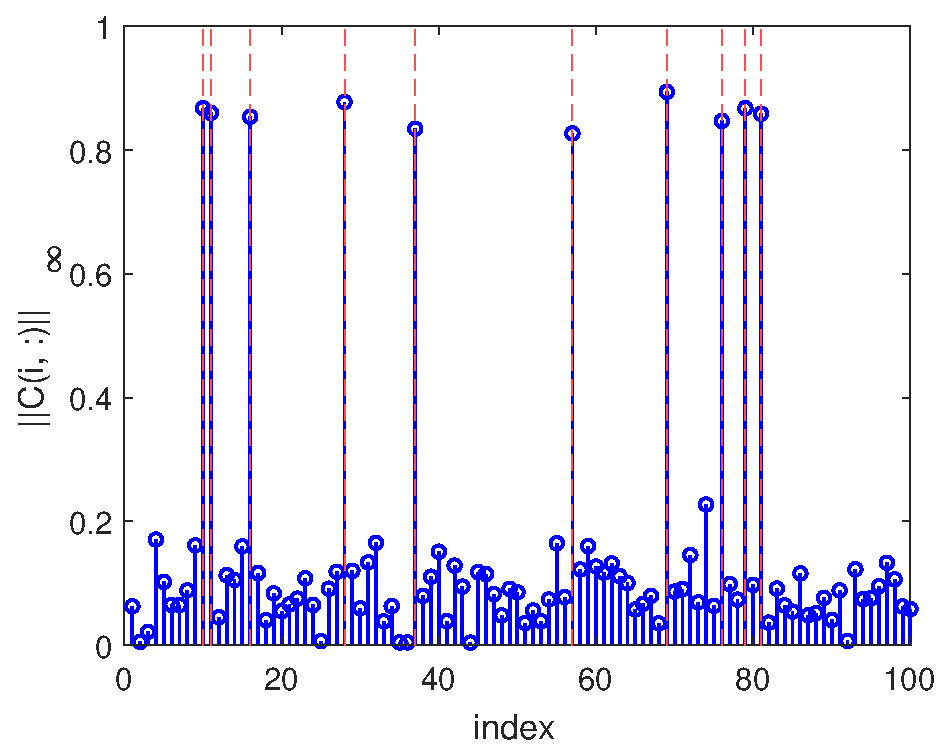
\includegraphics[width=0.4\textwidth]{figures/synthetic_data/unknown_K.eps}
%             \caption*{$M=50, K=10, N=100, \texttt{SNR}=20\text{dB}, \lambda=0.5$}
%         \end{figure}
%     \item However, the theorem does not speak for memory consumption.
% \end{itemize}
%
% \end{frame}

\begin{frame}
\frametitle{Memory}    
\begin{itemize}
    \item Recall the first step of FW is
        \[
        \bm{S} \leftarrow \argmin_{\bm{S} \in \mathcal{D}} \; \langle \nabla f(\bm{C}), \bm{S} \rangle
        \] 
    \item This sub-problem can be optimized on columns of $\bm{c}$'s independently
% \[
% f(\bm{C}) = \dfrac{1}{2}\norm{\bm{X} - \bm{X}\bm{C}}_{\rm F}^2 + \lambda \varPhi_{\mu}(\bm{C})
% \]
\[
\nabla f(\bm{C}) = \bm{X}^{\T}(\bm{X} - \bm{X}\bm{C}) + \lambda \nabla \varPhi_{\mu}(\bm{C})
\] 
\[
[\nabla \varPhi_{\mu}(\bm{C})]_{n,\ell} = \dfrac{\exp (c_{n, \ell}/\mu)}{\sum^{N}_{i=1} \exp(c_{n, i}/\mu)}
\] 
    \item Hence, memory requires for finding $\bm{S}$ in this step is $O(N)$
\end{itemize}

\begin{block}
    
    Will FW always find $ \bm{s}_\ell = \bm{e}_{n^{\star}}, \; n^{\star} \in \mathcal{K}$ for all $\ell \in [N]$?
\end{block}

    Yes, with some initialization strategy and noise is bounded by
    $ \delta \leq  \sqrt{\gamma^2 + \upsilon } -\gamma $ 
where 
\begin{align*}
&\upsilon= \lambda (1/N - \exp(\mu/\psi))/4 - D ,\\
&\psi = \min_{\substack{1 \leq i,j \leq N, \\ n \in \mathcal{K},  c^t_{n,i} \neq c^t_{n,j}}} \abs{c^t_{n,i} - c^t_{n, j}} 
\end{align*}
and $\gamma, D$ are some constants depending on  $\bm{W}, \bm{H}$

\note{
\begin{itemize}
    \item Increasing $\lambda$ to counter attack noise
\end{itemize}}
\end{frame}

\begin{frame}[label=current]
    \frametitle{Memory Intuition}
    \[
    %     \vphantom{% phantom stuff for correct box dimensions
    % \begin{matrix}
    % \overbrace{XYZ}^{\mbox{$R$}}\\ \\ \\ \\ \\ \\
    % \underbrace{pqr}_{\mbox{$S$}}
    % \end{matrix}}%
\begin{matrix}% matrix for left braces
\vphantom{a}\\
    \coolleftbrace{A}{e \\ y\\ y}\\
    \coolleftbrace{B}{y \\i \\ m}
\end{matrix}%
\begin{bmatrix}
a & \coolover{R}{b & c & d} & x & \coolover{Z}{x & x}\\
    e & f & g & h & x & x & x \\
    y & y & y & y & y & y & y \\
    y & y & y & y & y & y & y \\
    y & y & y & y & y & y & y \\
    i & j & k & l & x & x & x \\
    m & n & o  & p & x & x & x
\end{bmatrix}%
\begin{matrix}% matrix for right braces
    \coolrightbrace{x \\ x \\ y\\ y}{T}\\
    \coolrightbrace{y \\ y \\ x }{U}
\end{matrix}
\]
\[
\begin{matrix}% matrix for left braces
    \coolleftbrace{\mathcal{K}}{x \\ x\\ x} \\
    \coolleftbrace{\mathcal{K}^{c}}{x \\ x\\ x\\x} \\
\end{matrix}%
\begin{bmatrix}
 \tikzmarkx{left}{}&&\cdot&&&&  & & \cdot & \\
 &&\cdot&&&&  & & \cdot & \\
 &&\cdot&&&&  & & \cdot &\tikzmarkx{right}{} \\
 &&&&&& & & & \\
 &&&&&& & & & \\
 &&&&&& & & & \\
 &&&&&& & & & \\
 &&&&&& & & & \\
\end{bmatrix} 
\] 

%     \[
%         \vphantom{% phantom stuff for correct box dimensions
%     \begin{matrix}
%     \overbrace{XYZ}^{\mbox{$R$}}\\ \\ \\ \\ \\ \\
%     \underbrace{pqr}_{\mbox{$S$}}
%     \end{matrix}}%
% \begin{matrix}% matrix for left braces
% \vphantom{a}\\
%     \coolleftbrace{A}{e \\ y\\ y}\\
%     \coolleftbrace{B}{y \\i \\ m}
% \end{matrix}%
% \begin{bmatrix}
% a & \coolover{R}{b & c & d} & x & \coolover{Z}{x & x}\\
%     e & f & g & h & x & x & x \\
%     y & y & y & y & y & y & y \\
%     y & y & y & y & y & y & y \\
%     y & y & y & y & y & y & y \\
%     i & j & k & l & x & x & x \\
%     m &  \coolunder{S}{n & o}  & \coolunder{W}{p & x & x} & x
% \end{bmatrix}%
% \begin{matrix}% matrix for right braces
%     \coolrightbrace{x \\ x \\ y\\ y}{T}\\
%     \coolrightbrace{y \\ y \\ x }{U}
% \end{matrix}\]
\end{frame}
% \begin{frame}
% \frametitle{Memory}    
% \begin{theorem}[Regularized Case, Memory Efficiency]
% Assume that 
% \begin{itemize}
%     \item $\text{rank}(\bm{W})=K$
%     \item there exists at least an $n^\star \in \mathcal{K}$ such that $\bm{C}^t(n^\star,:)$ is not a constant row vector
%     \item The noise bound satisfies
%     $ \delta \leq  \sqrt{\gamma^2 + \upsilon } -\gamma $ 
% where 
% \begin{align*}
% &\gamma = \max_{k \in [K]} \norm{\bm{w}_k}_2, \\
% &\upsilon= \lambda (1/N - \exp(\mu/\psi))/4 - D ,\\
% &\psi = \min_{\substack{1 \leq i,j \leq N, \\ n \in \mathcal{K},  c^t_{n,i} \neq c^t_{n,j}}} \abs{c^t_{n,i} - c^t_{n, j}} 
% \end{align*}
% and $D$ is some constant depending on  $\bm{W}, \bm{H}$
% \end{itemize}
%
% If in iteration $t$, $\bm{C}^{t}$ satisfies ${\rm supp}(\bm{c}^{t}_\ell) \subseteq \mathcal{K}$ for all $\ell\in[N]$
% then, to attain $\bm{c}_\ell^{t+1}$ from $\bm{c}_\ell^t$, FW will update the $j_\ell$th element of $\bm{c}_\ell^t$ such that $j_\ell\in{\mathcal{K}}$ for all $\ell\in[N]$.
% \end{theorem}
% \end{frame}

% \begin{frame}
%     \frametitle{Initialization Condition}
%
% \begin{proposition}[Initialization Condition]
%     Let $\bm{C}^{\rm init}$ be a feasible initial solution. 
%     Define $$D_{ij}^n(\bm{C}) = \frac{t_{\rm init} (t_{\rm init}+1)}{2}\abs{c_{n,i} - c_{n,j}}$$ for some $t_{\rm init} \in \mathbb{N}, t_{\rm init}  \geq 1$.
%     Suppose that for some $ n^{\star} \in \mathcal{K}$, there exists a pair of $i^\star,j^\star$ such that {the following regularity condition is satisfied}:
%      \begin{equation*}
%          D_{i^\star j^\star}^{n^{\star}}(\bm{C}^{\rm init}) \notin \mathbb{N}.
%     \end{equation*} 
%     Running FW with $ \bm{C}^t=\bm{C}^{\rm init}$ starting with $t=t_{\text{init}}$ for $T$ iterations, the produced solution sequence $\set{\bm{C}}^{t}$ for $t \geq t_{\rm init}+1$ satisfies $\bm{C}^{t}(n^{\star}, :)$ is not a constant row vector and 
%     \[
%         \min_{\substack{{ n \in \mathcal{K},} i,j \\ c^t_{n,i} \neq c^t_{n,j}}}\abs{c^t_{n,i} - c^t_{n, j}} \geq \dfrac{2 \xi}{T(T+1)}
%     \]
%     where 
% $
%         \xi \coloneqq  \min_{
%         \substack{n \in \mathcal{K},i,j, 
%             z \in \mathbb{N} \\
%             D_{i,j}^n(\bm{C}^{\rm init}) \notin \mathbb{N}
%         }
%     } \abs{D_{i,j}^{n}(\bm{C}^{\rm init}) - z}.
% $ 
% \end{proposition}
% \end{frame}


\section{Experiment Demonstration}%
\label{sec:real_demonstration}

\subsection{Synthetic Data}%
\label{sub:synthetic}
\begin{frame}
    \frametitle{Synthetic Data}
    \begin{columns}
        \begin{column}{0.5\textwidth}
Data generation
\begin{itemize}
    \item $\bm{W} \sim \mathcal{U}(0, 1)$
    \item $\bm{H} \sim \text{Dir}(\bm{1}), \bm{H}(:, 1:K) = \bm{I}$
    \item $\bm{V} \sim \mathcal{N}(0, \sigma)$
    \item After shuffling $\bm{H}$, $\bm{X} = \bm{W} \bm{H} + \bm{V}$
    \item Noise level is measured in $\texttt{SNR}=10\log_{10} (\sum^{N}_{\ell=1} \norm{\bm{W}\bm{h}_\ell}_2^2)/(MN \sigma^2)$dB
\end{itemize}
Metric
\begin{itemize}
    \item \texttt{success rate} = $P(\mathcal{K} = \widehat{\mathcal{K}})$
    \item Estimate \texttt{success rate} by 50 trials
\end{itemize}
        \end{column}
        \begin{column}{0.65\textwidth}
            \vspace{-0.5cm}
\begin{figure}[!t]
    \centering
    \subfloat[Success rate under different SNRs; ${N =200}, M=50, K=40$.]{
    \label{fig:success_rate}
    \centering
    \begin{tikzpicture}[scale=0.48]
        \begin{axis}[
            /pgf/number format/1000 sep={},
            xlabel=\texttt{SNR},
            ylabel=\texttt{success rate},
            legend pos=south east,
            legend cell align={left},
            legend style={at={(0.52,0.01)}, anchor=south west,nodes={scale=0.9}},
            ]
        \addplot[purple,mark=+] table [x=SNR, y=SPA]{figures/synthetic_data/exp1/success_rate.dat};
        \addplot[orange,mark=o] table [x=SNR, y=FG]{figures/synthetic_data/exp1/success_rate.dat};
        \addplot[blue,mark=square] table [x=SNR, y=FW]{figures/synthetic_data/exp1/success_rate.dat};
        \legend{\texttt{SPA}, \texttt{FastGradient}, \texttt{MERIT}}
        \end{axis}
    \end{tikzpicture}
    }

    \subfloat[Memory consumption under different $N$'s;  $\text{SNR}=10\text{dB}, M=50, K=40$.]{
    \label{fig:mem}
    \centering
    \begin{tikzpicture}[scale=0.48]
        \begin{semilogyaxis}[
            /pgf/number format/1000 sep={},
            xlabel=$N$,
            ylabel=Memory cost in RSS (GB),
            legend pos=north west,
            legend cell align={left},
            xticklabel style={
                    /pgf/number format/fixed,
            },
            scaled x ticks=false,
            yticklabels={0., 0.1, 1.0},
            extra y ticks={0.3, 5.0},
            extra y tick labels={0.3, 5.0},
            extra tick style={tickwidth=\pgfkeysvalueof{/pgfplots/minor tick length}},
            ]
        \addplot[orange,mark=o] table [x=N, y=FG]{figures/synthetic_data/exp2/mem.dat};
        \addplot[blue,mark=square] table [x=N, y=FW]{figures/synthetic_data/exp2/mem.dat};
        \legend{\texttt{FastGradient}, \texttt{MERIT}}
        \end{semilogyaxis}
    \end{tikzpicture}
    }
    \caption*{Performance of \texttt{MERIT} compared to baselines}
\end{figure}
            
        \end{column}
    \end{columns}


\end{frame}

\subsection{Real data}%
\label{sub:real_data}
\begin{frame}
    \frametitle{Real Data: Topic Modeling}
    Metrics:
    \begin{itemize}
        \item \texttt{Coherence score} measures the quality of a mined topic. Higher score is better
        \item \texttt{Similarity count} is measured between topics. Smaller value is better
        \item \texttt{Accuracy} is measured using topic label. Higher score is better
    \end{itemize}
    Data
    \begin{itemize}
        \item TDT2
        \item Reuters-21578 
    \end{itemize}
\end{frame}

\begin{frame}
    \frametitle{Real Data: Topic Modeling}
\begin{table}
    \resizebox{\linewidth}{!}{\small
    \begin{tabular}{|p{1.2cm}|c|c|c|c|c|c|c|c|c|}
        \multicolumn{10}{c}{TDT2} \\
        \hline
        & \textbf{Method / $K$} & $3$ & $4$ & $5$ & $6$ & $7$ & $8$ & $9$ & $10$ \\
        \hline
        \multirow{6}{1.6cm}{Coherence $(\uparrow)$} 
        & \texttt{SPA} & {\blue -346.6} & -388.4 & -404.9 & -432.0 & -418.6 & -438.2 & -443.5 & -456.7 \\
        \cline{2-10}
        & \texttt{FastAnchor} & -468.6 & -483.4 & -483.3 & -495.9 & -525.8 & -536.2 & -546.5 & -543.2 \\
        \cline{2-10}
        & \texttt{XRAY} & -347.4 & -389.2 & -405.4 & -432.0 & -419.0 & -439.4 & -443.2 & -459.2 \\
        \cline{2-10}
        & \texttt{LDA} & -521.6 & -526.2 & -530.4 & -546.0 & -550.0 & -538.8 & -543.1 & -553.1 \\
        \cline{2-10}
        & \texttt{FastGradient} & -553.8 & -517.1 & -537.2 & -534.6 & -561.9 & -562.7 & -571.9 & -585.5 \\
        \cline{2-10}
         \rowcolor{green!10} & \texttt{MERIT} & -351.5 & \textbf{-375.7} & \textbf{-385.8} & \textbf{-394.4} & \textbf{-399.3} & \textbf{-417.2} & \textbf{-417.5} & \textbf{-429.1} \\
        \cline{2-10}
         % \rowcolor{green!10} & \texttt{MERIT(0)} & \textbf{-345.0} & {\blue -388.4} & {\blue -404.8} & -433.4 & -420.1 & -439.4 & -444.3 & -458.3  \\
        \hhline{|=|=|=|=|=|=|=|=|=|=|}
        \multirow{6}{1.6cm}{Similarity Count $(\downarrow)$}
        & \texttt{SPA} & {\blue 1.06} & 3.64   & 5.76   & 10.24  & 14.24  & 23.18  & 27.56  & 43.62  \\
        \cline{2-10}
        & \texttt{FastAnchor} & {\blue 1.06} & \textbf{2.02} & \textbf{3.90} & \textbf{4.80} & \textbf{6.18} & \textbf{7.98} & \textbf{9.92} & \textbf{11.22} \\
        \cline{2-10}
        & \texttt{XRAY} & \textbf{1.00} & 3.88 & 5.66 & 10.24& 14.16& 23.18& 28.00& 43.4 \\
        \cline{2-10}
        & \texttt{LDA} & 1.08 & {\blue 2.96} & {\blue 5.62} & {\blue 7.84} & {\blue 12.24}& {\blue 17.28}& {\blue 21.84}& {\blue 27.5} \\
        \cline{2-10}
        & \texttt{FastGradient} & 14.80 & 26.34 & 47.16 & 62.28 & 71.24 & 100.58& 109.84& 127.32 \\
        \cline{2-10}
        \rowcolor{green!10}& \texttt{MERIT} & 1.56 & 4.98 & 5.76 & 7.92 & 13.30 & 21.16 & 28.52 & 36.08 \\
        \cline{2-10}
          % \rowcolor{green!10}& \texttt{MERIT(0)} & 1.06 & 3.64 & 5.78 & 10.56 & 14.38 & 22.62 & 27.50 & 43.06 \\
        \hhline{|=|=|=|=|=|=|=|=|=|=|}
        \multirow{6}{1.6cm}{Accuracy $(\uparrow)$}
          & \texttt{SPA} & {\blue 0.87} & {\blue 0.83} & {\blue 0.81} & {\blue 0.81} & {\blue 0.78} & {\blue 0.76} & {\blue 0.75} & {\blue 0.72} \\
        \cline{2-10}
        & \texttt{FastAnchor} & 0.77 & 0.72 & 0.67 & 0.63 & 0.66 & 0.63 & 0.65 & 0.65  \\
        \cline{2-10}
        & \texttt{XRAY} & {\blue 0.87} & 0.82 & 0.80 & {\blue 0.81} & {\blue 0.78} & {\blue 0.75} & {\blue 0.75} & 0.71 \\
        \cline{2-10}
        & \texttt{LDA} & 0.78 & 0.77 & 0.74 & 0.75 & 0.73 & 0.72 & 0.68 & 0.70 \\
        \cline{2-10}
        & \texttt{FastGradient} & 0.70 & 0.71 & 0.65 & 0.64 & 0.61 & 0.56 & 0.58 & 0.57 \\
        \cline{2-10}
          \rowcolor{green!10} & \texttt{MERIT} & \textbf{0.88} & \textbf{0.88} & \textbf{0.85} & \textbf{0.86} & \textbf{0.84} & \textbf{0.82} & \textbf{0.80} & \textbf{0.77} \\
         \cline{2-10}
          % \rowcolor{green!10} & \texttt{MERIT}(0) & 0.86 & {\blue 0.83} & 0.80 & {\blue 0.81} & {\blue 0.78} & {\blue 0.76} & {\blue 0.75} & {\blue 0.72} \\
        \hline 
    \end{tabular}}
    \end{table}
\end{frame}

\begin{frame}
    \frametitle{Real Data: Topic Modeling}
\begin{table}
    \resizebox{\linewidth}{!}{\small
    \begin{tabular}{|p{1.2cm}|c|c|c|c|c|c|c|c|c|}
        \multicolumn{10}{c}{Reuters-21578} \\
        \hline
        & \textbf{Method / $K$} & $3$ & $4$ & $5$ & $6$ & $7$ & $8$ & $9$ & $10$ \\
        \hline
        \multirow{6}{1.6cm}{Coherence $(\uparrow)$}
        & \texttt{SPA} & {\blue -402.7} & -416.4 & \textbf{-420.5} & -442.1 & -516.5 & -520.3 & {\blue -541.5} & {\blue -548.3} \\
        \cline{2-10}
        & \texttt{FastAnchor} & -655.0 & -681.0 & -693.6 & -711.1 & - 757.5 & -827.7 & -832.8 & -843.4 \\
        \cline{2-10}
        & \texttt{XRAY} & -404.4 & {\blue -415.2} & -422.7 & {\blue -441.6} & {\blue -516.3} & {\blue -519.6} & -542.2 & -548.6 \\
        \cline{2-10}
        & \texttt{LDA} & -674.1 & -677.2 & -686.3 & -715.2 & -705.9 & -762.9 & -776.8 & -776.5 \\
        \cline{2-10}
        & \texttt{FastGradient} & -657.1 & -768.3 & -782.0 & -821.8 & -847.1 & -967.7 & -989.5 & -959.8 \\
        \cline{2-10}
          \rowcolor{green!10}& \texttt{MERIT} & -430.6 & -452.8 & -466.4 & -494.0 & -539.2 & -541.1 & -564.8 & -570.8 \\
        \cline{2-10}
        % \rowcolor{green!10}  & \texttt{MERIT(0)} & \textbf{-401.7} & \textbf{-413.3} & {\blue -422.5} & \textbf{-440.8} & \textbf{-511.2} & \textbf{-518.2} & \textbf{-536.0} & \textbf{-544.0} \\
        \hhline{|=|=|=|=|=|=|=|=|=|=|}
        \multirow{6}{1.6cm}{Similarity Count $(\downarrow)$}
        & \texttt{SPA} & 7.46 & 15.16 & 23.82 & 51.98 & 59.38 & 158.50 & 235.62 & 219.16 \\
        \cline{2-10}
        & \texttt{FastAnchor} & \textbf{5.40} & {\blue 8.46} & {\blue 13.06} & {\blue 20.06} & {\blue 25.56} & {\blue 42.28} & {\blue 54.9} & {\blue 57.84} \\
        \cline{2-10}
        & \texttt{XRAY} & 6.76 & 14.18 & 23.82 & 52.06 & 59.64 & 160.96 & 235.10 & 221.50 \\
        \cline{2-10}
        & \texttt{LDA} & \textbf{3.20} & \textbf{6.46} & \textbf{9.32} & \textbf{12.48} & \textbf{21.22} & \textbf{24.60} & \textbf{33.56} & \textbf{39.68} \\
        \cline{2-10}
        & \texttt{FastGradient} & 12.96  & 20.62  & 30.42  & 47.56  & 60.46  & 82.86  & 106.66 & 144.38 \\
        \cline{2-10}
        \rowcolor{green!10} & \texttt{MERIT} & 7.34 & 16.04 & 21.88 & 36.08 & 48.36 & 93.32 & 131.62 & 141.42 \\
        \cline{2-10}
        % \rowcolor{green!10} & \texttt{MERIT(0)} & 7.38 & 15.18 & 23.24 & 45.12 & 54.60 & 145.52 & 223.66 & 214.60 \\
        \hhline{|=|=|=|=|=|=|=|=|=|=|}
        \multirow{6}{1.6cm}{Accuracy $(\uparrow)$}
          & \texttt{SPA} & {\blue 0.64} & 0.57 & {\blue 0.54} & 0.51 & 0.49 & 0.44 & 0.42 & 0.40 \\
        \cline{2-10}
        & \texttt{FastAnchor} & 0.60 & 0.57 & 0.52 & {\blue 0.52} & 0.46 & 0.42 & 0.38 & 0.37 \\
        \cline{2-10}
        & \texttt{XRAY} & 0.63 & 0.57 & {\blue 0.54} & 0.51 & 0.49 & {\blue 0.45} & 0.42 & 0.40 \\
        \cline{2-10}
        & \texttt{LDA} & 0.63 & 0.57 & 0.53 & 0.51 & 0.46 & 0.44 & 0.41 & 0.42 \\
        \cline{2-10}
        & \texttt{FastGradient} & 0.62 & 0.57 & \textbf{0.56} & 0.51 & {\blue 0.50} & \textbf{0.48} & \textbf{0.44} & \textbf{0.46} \\
        \cline{2-10}
        \rowcolor{green!10}   & \texttt{MERIT} & \textbf{0.66} & \textbf{0.62} & 0.53 & \textbf{0.53} & \textbf{0.51} & \textbf{0.48} & {\blue 0.43} & {\blue 0.45} \\
        \cline{2-10}
         % \rowcolor{green!10}  & \texttt{MERIT(0)} & {\blue 0.64} & {\blue 0.58} & {\blue 0.54} & {\blue 0.52} & 0.49 & 0.44 & 0.42 & 0.41 \\
        \hline 
    \end{tabular}
}
    \end{table}
\end{frame}
\begin{frame}
    \frametitle{Real Data: Topic Modeling}
% \begin{figure}[t]
%     \centering
%     \subfloat[TDT2] {
%         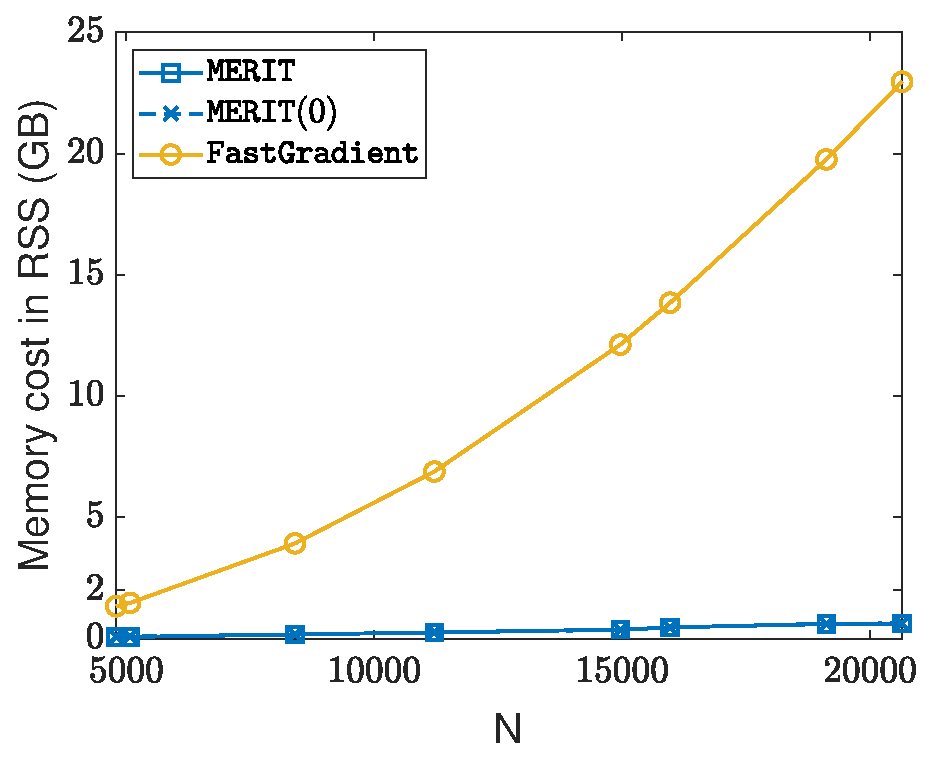
\includegraphics[width=0.35\textwidth]{figures/topic_modeling/tdt2/tdt2_mem.eps}
%         \label{fig:topic_mem_tdt2}
%     }
%     \subfloat[Reuters-21578] {
%         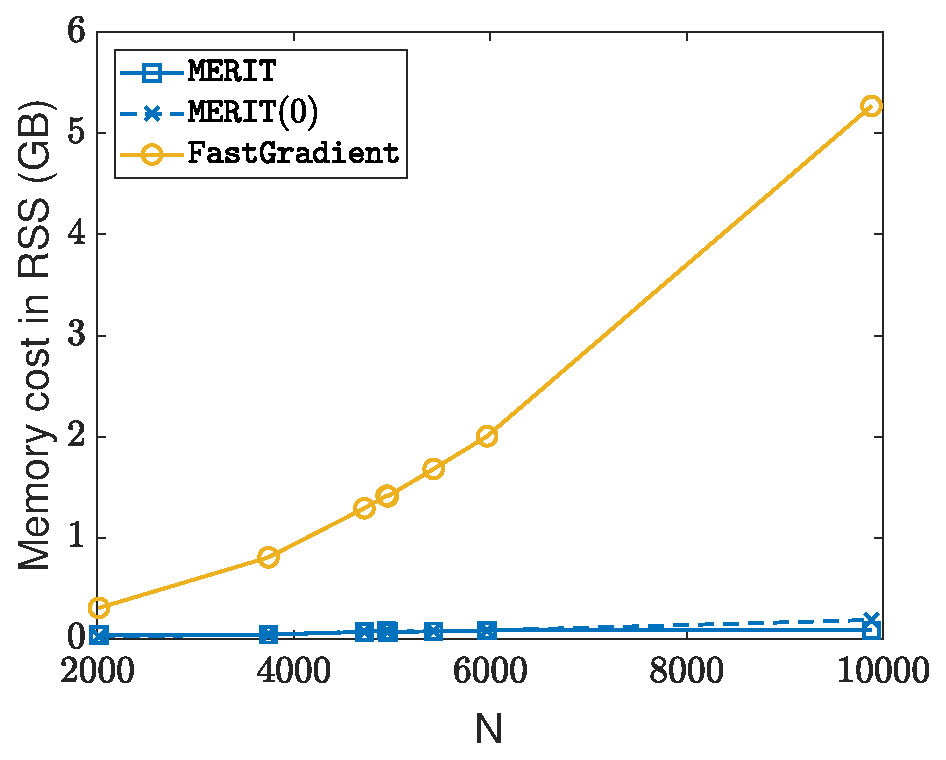
\includegraphics[width=0.35\textwidth]{figures/topic_modeling/reuters/reuters_mem.eps}
%         \label{fig:topic_mem_reuters}
%     }
%     \caption*{Memory consumption of \texttt{FastGradient} and \texttt{MERIT}, under different sample sizes.}
%     \label{fig:topic_mem}
% \end{figure}

\begin{figure}[t]
    \centering
    \begin{subfigure}{0.45\textwidth}
    \begin{tikzpicture}[scale=0.55]
        \begin{axis}[
            /pgf/number format/1000 sep={},
            xlabel=$N$,
            ylabel=Memory cost in RSS (GB),
            legend pos=north west,
            legend cell align={left},
            ]
        \addplot[orange,mark=o] table [x=N, y=FG]{figures/topic_modeling/tdt2/mem.dat};
        \addplot[blue,mark=square] table [x=N, y=FW]{figures/topic_modeling/tdt2/mem.dat};
        \legend{\texttt{FastGradient}, \texttt{MERIT}}
        \end{axis}
    \end{tikzpicture}
    % \captionsetup{justification=centering,margin=0.2cm,font=scriptsize}
    \caption*{TDT2} 
    \end{subfigure}
    \begin{subfigure}{0.45\textwidth}
    \begin{tikzpicture}[scale=0.55]
        \begin{axis}[
            /pgf/number format/1000 sep={},
            xlabel=$N$,
            ylabel=Memory cost in RSS (GB),
            legend pos=north west,
            legend cell align={left},
            ]
        \addplot[orange,mark=o] table [x=N, y=FG]{figures/topic_modeling/reuters/mem.dat};
        \addplot[blue,mark=square] table [x=N, y=FW]{figures/topic_modeling/reuters/mem.dat};
        \legend{\texttt{FastGradient}, \texttt{MERIT}}
        \end{axis}
    \end{tikzpicture}
    \captionsetup{justification=centering,margin=0.2cm,font=scriptsize}
    \caption*{Reuters-21578} 
    \end{subfigure}
    % \captionsetup{justification=centering,margin=0.2cm,font=scriptsize}
    \caption*{Memory consumption of \texttt{FastGradient} and \texttt{MERIT}} 
\end{figure}

\note{
    \begin{itemize}
        \item Discuss about baselines
    \end{itemize}
}
\end{frame}

\begin{frame}
    \frametitle{Real Data: Community detection}
    \begin{itemize}
        \item Metric: Spearman's rank correlation (SRC). SRC $\in [-1, 1]$, higher value is better.
        \item Data: co-authorship networks, a community ground truth is defined by
        \begin{itemize}
            \item DBLP:  group of conferences
            \item MAG: ``field of study'' tag
        \end{itemize}
    \end{itemize}
    \begin{columns}
        \begin{column}{0.5\textwidth}
\begin{table}[!t]
    \centering
    \vspace{0.7cm}
        \resizebox{\linewidth}{!}{\large
        \begin{tabular}{|c|c|c|c|c|}
            \hline
            \textbf{Dataset}   &   \texttt{GeoNMF} & \texttt{SPOC} &  \texttt{FastGradient} & \texttt{MERIT}   \\  \hline \hline
            DBLP1 &  0.2974 & {\blue 0.2996} &  \textbf{0.3145} & 0.2937 \\
            DBLP2 &  0.2948 & 0.2126 &  {\blue 0.3237} & \textbf{0.3257}  \\
            DBLP3 &  0.2629 & \textbf{0.2972} &  0.1933 & {\blue 0.2763}  \\
            DBLP4 &  0.2661 & {0.3479} &  0.1601 & \textbf{0.3559}  \\
            DBLP5 &  {\blue 0.1977} & 0.1720 &  0.0912 & \textbf{0.1983}  \\
            MAG1  &  \textbf{0.1349} & {\blue 0.1173} &  0.0441 & 0.1149  \\
            MAG2  & 0.1451& 0.1531 & {\bf 0.2426} & {\blue 0.2414} \\
            \hline
        \end{tabular}}
        \vspace{0.5cm}
    \caption*{SRC Performance on DBLP and MAG}
\end{table}
        \end{column}
        \begin{column}{0.55\textwidth}
\begin{figure}[t]
    \centering
    \vspace{-0.6cm}
    \begin{tikzpicture}[scale=0.55]
        \begin{axis}[
            /pgf/number format/1000 sep={},
            xlabel=$N$,
            ylabel=Memory cost in RSS (GB),
            legend pos=north west,
            legend cell align={left},
            ]
        \addplot[orange,mark=o] table [x=N, y=FG]{figures/community_detection/mem.dat};
        \addplot[blue,mark=square] table [x=N, y=FW]{figures/community_detection/mem.dat};
        \legend{\texttt{FastGradient}, \texttt{MERIT}}
        \end{axis}
    \end{tikzpicture}
    \captionsetup{justification=centering,margin=0.2cm,font=scriptsize}
    \caption*{Memory consumption of \texttt{FastGradient} and \texttt{MERIT}} 
\end{figure}
        \end{column}
    \end{columns}
\end{frame}

\begin{frame}
    \frametitle{Conclusion}
    \begin{itemize}
        % \item Separable NMF has been tacked by 2 main approaches: greedy methods and convex relaxation algorithms
        % \item Greedy methods suffer from error propagation, while convex relaxation algorithms is limited by its huge memory requirement
        \item FW is proposed as a memory efficient method for convex relaxation approach to tackle separable NMF
        \item When noise is absent, using FW can bring identification with memory $O(KN)$
        \item For noisy case, we proposed using a smooth regularization to guarantee identification
        \item For noisy case, we also shown that running FW only cost $O(KN)$ using some initialization strategy
    \end{itemize}
\end{frame}

% \begin{frame}
%     \frametitle{Future Work: Zero-Inflation Community Detection}
%     \begin{align*}
%     &\bm{P} = \bm{M} \bm{B} \bm{M}^{\T} , \\
%     &O_{ij} \sim \text{Bernoulli}(P_{ij}) \\
%     &D_{ij} \sim \text{Bernoulli}(T_{ij}) \\
%     &A_{ij} = \begin{cases}
%         O_{ij} \quad & \text{if } D_{ij} = 1 \\
%         0 & \text{otherwise}
%     \end{cases}
%     \end{align*}
%     Given the observations $A_{ij}, (i,j) \in \Omega$, we hope to estimate $\bm{M}, \bm{B}$.
% \end{frame}

\begin{frame}[allowframebreaks]
    \frametitle{Reference}
    { \footnotesize
    \printbibliography}
\end{frame}


\end{document}
